\documentclass[reqno]{amsart}
\usepackage[utf8]{inputenc}
\usepackage[margin=1in]{geometry}
\usepackage[usenames, dvipsnames]{xcolor}
\usepackage{graphicx}
\usepackage{mathtools}
\usepackage{amssymb}
\usepackage{amsthm}
\usepackage{fancyhdr}
\usepackage{adforn}
\usepackage{xparse}
\usepackage{tikz}
\usetikzlibrary{fadings}
%\usetikzlibrary{matrix, positioning, calc}
% Additional math macros that I want in both my notes and my psets
\usepackage[sc, noBBpl]{mathpazo}
\usepackage{mathrsfs}
\usepackage[T1]{fontenc}
\usepackage{calligra}
\usepackage{microtype}
\usepackage[all]{xy}
\usepackage{slashed}
\newcommand{\A}{\mathbb A}
\newcommand{\cat}{\mathsf}
\newcommand{\sC}{\cat C}
\newcommand{\sD}{\cat D}
\newcommand{\sS}{\cat S}
\newcommand{\sA}{\mathscr A}
\newcommand{\sF}{\mathscr F}
\newcommand{\sG}{\mathscr G}
\renewcommand{\P}{\mathbb P}
\newcommand{\cO}{\mathscr O}
\newcommand{\sI}{\mathscr I}
\DeclareMathOperator{\coker}{coker}
\renewcommand{\Im}{\operatorname{Im}}
\newcommand{\pt}{\mathrm{pt}}
\DeclareMathOperator{\Hom}{Hom}
\newcommand{\op}{^{\mathsf{op}}}
\newcommand{\Id}{\mathrm{Id}}
\DeclareMathOperator{\Mat}{Mat}
\newcommand{\m}{\mathfrak m}
%\newcommand{\p}{\mathfrak p}
\newcommand{\q}{\mathfrak q}
\DeclareMathOperator{\MSpec}{MSpec}
\DeclareMathOperator{\Spec}{Spec}
\newcommand{\Top}{\cat{Top}}
\newcommand{\Ring}{\cat{Ring}}
\newcommand{\Mod}{\cat{Mod}}
\DeclareMathOperator{\res}{res}
\newcommand{\Alg}{\cat{Alg}}
\newcommand{\Fun}{\cat{Fun}}
\newcommand{\AffSch}{\cat{AffSch}}
\newcommand{\Ab}{\cat{Ab}}
\DeclareMathOperator{\bl}{--}
\DeclareMathOperator{\Free}{Free}
\DeclareMathOperator{\For}{For}
\newcommand{\Set}{\cat{Set}}
\newcommand{\LocRing}{\cat{LocRing}}
\newcommand{\Grp}{\cat{Grp}}
\newcommand{\Sch}{\cat{Sch}}
\newcommand{\inHom}{\operatorname{\underline{\Hom}}}
\DeclareMathOperator{\Frac}{Frac}
\DeclareMathOperator{\Gal}{Gal}
\DeclareMathOperator{\Nil}{Nil}
\newcommand{\pre}{\sC^{\text{pre}}}
\newcommand{\sh}{_{\text{sh}}}
\newcommand{\G}{\mathbb G}
\DeclareMathOperator{\Proj}{Proj}
\newcommand{\sM}{\mathscr M}
\newcommand{\sV}{\mathscr V}
\newcommand{\fU}{\mathfrak U}
\newcommand{\GL}{\mathrm{GL}}
\DeclareMathOperator{\Sym}{Sym}
% http://tex.stackexchange.com/questions/141434/how-to-type-sheaf-hom
\DeclareMathOperator{\shom}{\mathscr{H}\text{\kern -4pt {\calligra\large om}}\,}
\newcommand{\sL}{\mathscr L}
\DeclareMathOperator{\QC}{QC}
\DeclareMathOperator{\Supp}{Supp}
\newcommand{\sN}{\mathscr N}
\DeclareMathOperator{\Ann}{Ann}
\DeclareMathOperator{\Der}{Der}
\newcommand{\ctcpx}[1]{(#1)^{\text{der}}}
\newcommand{\Dist}{\mathsf{Dist}}
\newcommand{\shdi}{\operatorname{Sh}_{\Dist}}
\DeclareMathOperator{\Sh}{Sh}
\newcommand{\shz}{\mathsf{Sh}_{\text{\rm Zar}}}
\DeclareMathOperator{\Gr}{Gr}
% Source: http://tug.org/pipermail/xy-pic/2001-July/000015.html
\newcommand{\pullbackcorner}[1][dr]{\save*!/#1+1.2pc/#1:(1,-1)@^{|-}\restore}
\newcommand{\pushoutcorner}[1][dr]{\save*!/#1-1.2pc/#1:(-1,1)@^{|-}\restore}
\newcommand{\TDel}{\mathrm{2\Delta}}
\DeclareMathOperator{\Bl}{B\ell}
\newcommand{\cR}{\mathcal R}
\newcommand{\cL}{\mathcal L}
\newcommand{\cH}{\mathcal H}
\newcommand{\refR}{\reflectbox{\(\cR\)}}

\renewcommand{\a}{\alpha}
\renewcommand{\b}{\beta}
%\newcommand{\e}{\epsilon}
\renewcommand{\l}{\lambda}
\renewcommand{\L}{\Lambda}
\newcommand{\g}{\gamma}
\newcommand{\s}{\sigma}
\newcommand{\z}{\zeta}
\newcommand{\RR}{\mathbb{R}}
\newcommand{\NN}{\mathbb{N}}
\newcommand{\QQ}{\mathbb{Q}}
\newcommand{\ZZ}{\mathbb{Z}}
\newcommand{\CC}{\mathbb{C}}
\newcommand{\cC}{\mathcal{C}}
\newcommand{\f}{\frac}
\newcommand{\p}{\partial}
\renewcommand{\P}[3][]{\f{\partial^{#1} #2}{\partial #3 ^{#1}}}
%\newcommand{\avg}[1]{\langle #1 \rangle}
\newcommand{\avg}[1]{\left< #1 \right>}
\newcommand{\?}{\overset{?}{=}}
\newcommand{\Int}{\int_{-\infty}^\infty}
\newcommand{\ket}[1]{\left| #1 \right>} % for Dirac bras
\newcommand{\bra}[1]{\left< #1 \right|} % for Dirac kets
\newcommand{\braket}[2]{\left< #1 \vphantom{#2} \right|
 \left. #2 \vphantom{#1} \right>} % for Dirac brackets
\newcommand{\pv}{\vec{p}}

\newcommand{\grad}[1]{\gv{\nabla} #1} % for gradient
\let\divsymb=\div % rename builtin command \div to \divsymb
\renewcommand{\div}[1]{\gv{\nabla} \cdot #1} % for divergence
\newcommand{\curl}[1]{\gv{\nabla} \times #1} % for curl
\renewcommand{\labelenumi}{(\alph{enumi})}
\let\vaccent=\v % rename builtin command \v{} to \vaccent{}
\renewcommand{\v}[1]{\ensuremath{\mathbf{#1}}}
\newcommand{\uv}[1]{\ensuremath{\mathbf{\hat{#1}}}} % for unit vector
\newcommand{\gv}[1]{\ensuremath{\mbox{\boldmath$ #1 $}}} 
% for vectors of Greek letters
\usepackage{hyperref}
\usepackage{siunitx}

%\usepackage[compat=1.1.0]{tikz-feynman}

% TODO fiddle with colors
\definecolor{newblue}{HTML}{1F98A6}
\definecolor{newred}{HTML}{D95448}
\definecolor{neworange}{HTML}{F29441}
\hypersetup{
	colorlinks,
	linkcolor=newred,
	citecolor=neworange,
	urlcolor=newblue!80!black,
}
\usepackage[all]{hypcap}
\pagestyle{plain}
\setcounter{tocdepth}{1}


\usepackage{titlesec}
\titleformat{\section}[frame]
  {\normalfont}
  {\filright
   \footnotesize
   \enspace Lecture \arabic{section}.\enspace}
  {8pt}
  {\Large\bfseries\filcenter}
\usepackage[dotinlabels]{titletoc}
\titlecontents{section}[1.5em]{}{\contentslabel{2.3em}}{\hspace*{-2.3em}}{\hfill\contentspage}

\renewcommand{\sectionmark}[1]{\markleft\thesection. #1}

\fancyhf{}
\fancyhead[RO,LE]{\small\thepage}
\fancyhead[LO]{\small\slshape\nouppercase{\rightmark}}
\fancyhead[RE]{\small\slshape Advanced Quantum Field Theory Lecture Notes}
\setlength{\headheight}{11.0pt}
\pagestyle{fancy}

\numberwithin{equation}{section}
\newcommand{\orbreak}{
\begin{center}
	\adforn{17}\;\(\cdot\)\;\adforn{18}
	\vspace{0.2cm}
\end{center}
}

\renewcommand{\labelitemi}{\(\circ\)}

% I wanted to allow one to reference parts of a thm/cor/etc. and have it print the thm number too, e.g. 29.2(1),
% but this isn't working right now. Probably the best way to do this would be to play around with enumitem to
% define a new enumerate-like counter and then just use that directly instead of enumerate in comp.

% This feels really wobbly, but so far it's working
\NewDocumentEnvironment{comp}{mm}{%
	\csname #1\endcsname\hfill
	\csname #2\endcsname
}{
	\csname end#2\endcsname
	\csname end#1\endcsname
}

% usage:
% \shortexact[f][g]{A}{B}{C},
%
%			 f    g
% for 0 -> A -> B -> C -> 0,
\DeclareDocumentCommand{\shortexact}{O{} O{} mmmm}{
\xymatrix{
	0\ar[r] & #3\ar[r]^-{#1} & #4\ar[r]^-{#2} & #5\ar[r] & 0#6
}}
% exactly the same, but for 0 -> A -> B -> C
\DeclareDocumentCommand{\leftexact}{O{} O{} mmmm}{
\xymatrix{
	0\ar[r] & #3\ar[r]^-{#1} & #4\ar[r]^-{#2} & #5 #6
}}
% ... and the same, for A -> B -> C -> 0
\DeclareDocumentCommand{\rightexact}{O{} O{} mmmm}{
\xymatrix{
	#3\ar[r]^-{#1} & #4\ar[r]^-{#2} & #5\ar[r] & 0#6
}}



% usage:
% X\dblarrow[r] & Y
%   f
% X => Y
%   g
\DeclareDocumentCommand{\dblarrow}{O{} O{} O{}}{
	\ar@<0.4ex>[#1]^-{#2}\ar@<-0.4ex>[#1]_-{#3}
}
% Note: it would be a useful exercise to figure out how to define this so it can be used as
% \dblarrow[r]^f_g

\everyentry={\displaystyle}

\newcommand{\N}{\mathbb N}
\newcommand{\Z}{\mathbb Z}
\newcommand{\Q}{\mathbb Q}
\newcommand{\R}{\mathbb R}
\newcommand{\C}{\mathbb C}
\newcommand{\F}{\mathbb F}
\newcommand{\vp}{\varphi}
\newcommand{\term}{\emph}
\renewcommand{\vec}[1]{\boldsymbol{\mathbf{#1}}}
\DeclarePairedDelimiter\paren{(}{)}
%\DeclarePairedDelimiter\ang{\langle}{\rangle}
\DeclarePairedDelimiter\abs{\lvert}{\rvert}
\DeclarePairedDelimiter\norm{\lVert}{\rVert}
\DeclarePairedDelimiter\bkt{[}{]}
\DeclarePairedDelimiter\set{\{}{\}}
% Swap paren* and paren, etc., so that the normal version resizes by default.
% Meanwhile, one can use \paren*[\Big]{...} to customize the size easily.
% It would be interesting to wrap this up into a custom \definedelimiter command...
\makeatletter
	\let\oldparen\paren
	\def\paren{\@ifstar{\oldparen}{\oldparen*}}
	\let\oldbkt\bkt
	\def\bkt{\@ifstar{\oldbkt}{\oldbkt*}}
\makeatother
\newcommand{\e}{\varepsilon}
\def\qedsymbol{{\small{\ensuremath{\boxtimes}}}}
\newcommand{\inj}{\hookrightarrow}
\newcommand{\surj}{\twoheadrightarrow}
\DeclareMathOperator{\id}{id}
\newcommand{\ud}{\,\mathrm{d}}
\renewcommand{\d}{\mathrm d}
\newcommand{\dfr}[2]{\frac{\mathrm d #1}{\mathrm d #2}}
\newcommand{\pfr}[2]{\frac{\partial #1}{\partial #2}}

%\catcode`\"=13
%\newcommand{"}[1]{^{(#1)}}
\newtheorem{thm}[equation]{Theorem}
\newtheorem*{thm*}{Theorem}
\newtheorem{lem}[equation]{Lemma}
\newtheorem*{lem*}{Lemma}
\newtheorem{cor}[equation]{Corollary}
\newtheorem{prop}[equation]{Proposition}
\newtheorem{obs}[equation]{Observation}
\theoremstyle{definition}
\newtheorem{ex}[equation]{Exercise}
\newtheorem{exm}[equation]{Example}
\newtheorem{defn}[equation]{Definition}
\newtheorem*{claim}{Claim}
\theoremstyle{remark}
\newtheorem*{rem}{Remark}
\newtheorem*{fct}{Fact}
\newtheorem*{note}{Note}

\begin{document}
\title{Advanced Quantum Field Theory}
\author{Ian Lim\\ Last updated \today}
\maketitle
{\small\noindent These notes were taken for the \textit{Advanced Quantum Field Theory} course taught by Matthew Wingate at the University of Cambridge as part of the Mathematical Tripos Part III in Michaelmas Term 2018. I live-\TeX ed them using Overleaf, and as such there may be typos; please send questions, comments, complaints, and corrections to 
\href{mailto:itel2@cam.ac.uk?subject=AQFT\%20Lecture\%20Notes}{\texttt{itel2@cam.ac.uk}}.\\
Many thanks to Arun Debray for the {\LaTeX} template for these lecture notes: as of the time of writing, you can find him at \url{https://web.ma.utexas.edu/users/a.debray/}.}

\tableofcontents

\section{Saturday, January 19, 2019}
	\begin{note}
There will not be official typed course notes, but there will be scanned handwritten notes (which I will link here as they become available). Previous lecturers' notes are currently online (Skinner, Osborn).
\end{note}

Today we introduce path integrals in a QFT context. There are some benefits to working with path integrals-- some computations are simplified or more straightforward, and Lorentz invariance is manifest (unlike in the canonical formalism).

\subsection*{Path integrals in quantum mechanics} Rather than trying to tackle the full machinery of QFT, we'll start with $0+1$ dimensional non-relativistic quantum mechanics (cf. Osborn $\mathsection$ 1.2. We'll set $\hbar = 1$ for now, though we may restore it later in order to make arguments when $\hbar \ll 1$ in a classical limit. In these units,
\begin{equation*}
    [E][t]=[\hbar]=[p][x]
\end{equation*}
using uncertainty relations.

Let us consider a Hamiltonian in $1$ spatial dimension,
\begin{equation*}
    \hat H=H(\hat x, \hat p)\quad \text{with }[\hat x,\hat p]=i.
\end{equation*}
We'll further assume for simplicity that the Hamiltonian has a kinetic term and a potential based only on position,
\begin{equation*}
    \hat H= \frac{\hat p^2}{2m}+V(\hat x).
\end{equation*}

Now the Schr\"odinger equation takes the form
\begin{equation}
    i\P{}{t}\ket{\psi(t)}=\hat H \ket{\psi(t)}
\end{equation}
which has formal solution
\begin{equation}\label{schrodingerformal}
    \ket{\psi(t)}=e^{-i\hat H t}\ket{\psi(0)}.
\end{equation}
Let us consider some position eigenstates $\ket{x,t}$ such that
\begin{equation*}
    \hat x(t)\ket{x,t}=x \ket{x,t},\quad x\in \RR,
\end{equation*}
where these states obey some normalization
\begin{equation*}
    \braket{x',t}{x,t}=\delta(x'-x).
\end{equation*}
In the Schr\"odinger picture, states depend on time, while operators are constant. In terms of fixed (time-independent) eigenstates $\set{\ket{x}}$ of the position operator $\hat x$, we may write the wavefunction as
\begin{equation}
    \psi(x,t)=\braket{x}{\psi(t)},
\end{equation}
so that applying the Hamiltonian to the wavefunction $\psi(x,t)$ yields
\begin{equation}
    \hat H \psi(x,t)=(-\frac{1}{2m}\frac{\p^2}{\p x^2} + V(x))\psi(x,t).
\end{equation}

This is the traditional presentation of quantum mechanics and the wavefunction. In the path integral formalism, we'll consider a more particle-like treatment, where we express time evolution as a sum over all trajectories (meeting some boundary conditions) appropriately weighted (by an action).

Recall that our formal solution \ref{schrodingerformal} tells us what $\ket{\psi(t)}$ is-- we can therefore rewrite the wavefunction as
\begin{equation}
    \psi(x,t)\bra{x}e^{-i\hat Ht} \ket{\psi(0)}.
\end{equation}
By inserting a complete set of (position eigen)states, $1=\int dx_0 \ket{x_0}\bra{x_0}$, we get
\begin{align*}
    \psi(x,t) &=\int dx_0 \bra{x} e^{-i\hat Ht}\ket{x_0} \braket{x_0}{\psi(0)}\\
        &= \int dx_0\, K(x,x_0; t) \psi(x_0,0),
\end{align*}
where we have defined $K(x,x_0;t) \equiv \bra{x} e^{-i\hat Ht}\ket{x_0}$. Let us further consider time evolution in discrete steps, with $0\equiv t_0 < t_1 < t_2 < \ldots < t_n < t_{n+1} \equiv T$ so that
\begin{equation*}
    e^{-i\hat H T}= e^{-i\hat H(t_{n+1}-t_n)} \ldots e^{-i\hat H (t_1-t_0)}.
\end{equation*}
As before, we insert complete sets of states, finding that our generic time evolution from any $x_0$ to an $x$ of our choosing:
\begin{equation}
    K(x,x_0;T) = \int \left[ \prod_{r=1}^n dx_r \bra{x_{r+1}} e^{-i\hat H(t_{r+1}-t_r)}\ket{x_r}\right] \bra{x_1}e^{-i\hat H t_1}\ket{x_0}.
\end{equation}
That is, we integrate over all intermediate positions $x_r$ for each $t_r$. Naturally, $dx_{n+1}$ must be $x$.

Let's look at the free theory first to understand what we've done, $V(x)=0$. Now this weird $K_0$ object we've defined takes the form
\begin{equation}
    K_0(x,x'; t)=\bra{x}e^{-i \frac{\hat p^2}{2m} t}\ket{x'}.
\end{equation}
We'll instead insert a complete set of momentum eigenstates $\ket{p}$ with the normalization
\begin{equation*}
    \int \frac{dp}{2\pi}\ket{p}\bra{p}=1,
\end{equation*}
recalling that $\braket{x}{p}=e^{ipx}$ are simply plane waves. Then
\begin{equation*}
    K_0 (x,x'; t)=\int \frac{dp}{2\pi} e^{-i p^2 t/2m} e^{ip (x-x')}.
\end{equation*}
We can compute this-- completing the square with a change of variables to $p'=p- \frac{m(x-x')}{t}$, $K_0$ becomes a gaussian integral,
\begin{align*}
    K_0(x,x';t) &= e^{im(x-x')^2/2t} \int_{-\infty}^\infty \exp \left[-\frac{i(p')^2 t}{2m}\right]\\
    &= e^{im(x-x')^2/2t} \sqrt{\frac{m}{2\pi i t}}.
\end{align*}
Note that as $t\to 0$,%
    \footnote{This was more obvious from the original expression for $K_0$ where $K_0(x,x'; t=0)= \int \frac{dp}{2\pi} e^{ip(x-x')}.$}
\begin{equation*}
    \lim_{t\to 0} K_0(x,x'; t)=\delta(x-x'),
\end{equation*}
which agrees with the fact that $\braket{x'}{x}=\delta(x-x')$.

For $V(\hat x)\neq 0$, we still need small time steps but since operators generically do not compute, exponentials don't add in the usual way:
\begin{equation*}
    e^{\hat A} e^{\hat B} = \exp(\hat A + \hat B + \frac{1}{2}[\hat A, \hat B] + \ldots) \neq e^{\hat A + \hat B}\quad \text{when }[\hat A, \hat B] \neq 0.
\end{equation*}
This is the Baker-Campbell-Hausdorff (BCH) formula. However, for small $\epsilon$ we can write
\begin{equation*}
    e^{\epsilon \hat A} e^{\epsilon \hat B} = \exp(\epsilon \hat A + \epsilon \hat B +O(\epsilon^2)),
\end{equation*}
or equivalently
\begin{equation*}
    e^{\epsilon(\hat A + \hat B)} = e^{\epsilon \hat A} e^{\epsilon \hat B}(1+O(\epsilon^2)),
\end{equation*}
so we conclude that
\begin{equation*}
    e^{\hat A +\hat B}=\lim_{n\to \infty} \left(e^{\hat A/n}e^{\hat B/n}\right)^n.
\end{equation*}

Suppose now that we divide our time into $n$ time steps so that $t_r-1-t_r=\delta t$, with $T=n\delta t$. Then one of the intermediate time evolution steps looks like
\begin{align*}
    \bra{x_{r+1}} e^{-i\hat H \delta t}\ket{x_r}
        &= e^{-iV(x_r)\delta t} \bra{x_{r+1}} e^{-i\hat p^2 \delta t/2m} \ket{x_r}\\
        &= \sqrt{\frac{m}{2\pi i \delta t}} \exp\left[\frac{i}{2} m\left(\frac{x_{r+1}-x_r}{\delta t}\right)^2 \delta t - i V(x_r)\delta t\right].
\end{align*}
Taking $T=n\delta t,$ we find that the entire $K$ becomes
\begin{equation}
    K(x,x_0; T) =\int \left( \prod^n_{r=1} dx_r\right) \left(\frac{m}{2\pi i \delta t}\right)^{\frac{n+1}{2}} \exp \left( i\sum_{r=0}^n \left[\frac{m}{2}\left(\frac{x_{r+1}-x_r}{\delta t}\right)^2 -V(x_r)\right]\delta t\right).
\end{equation}
Now we take the limit as $n\to \infty, \delta t\to 0$ with $T$ fixed. Then the argument of the exponential becomes
\begin{equation}
    \int_0^T \frac{m}{2} \dot x^2 - V(x)] dt = \int_0^t L dt,
\end{equation}
where $L(x,\dot x)$ is the classical Lagrangian and this integral is nothing more than the action. We conclude that
\begin{equation}
    K(x,x_0;T) = \bra{x} e^{-i\hat H t}\ket{x_0} = \int \mathcal{D}x\, e^{iS[x]},
\end{equation}
where $S[x]=\int_0^T L(x, \dot x) dt$ is the classical action and the $\mathcal{D}$ conceals all our sins (the continuum limit) in a cute integration measure. Note that the action has units of energy$\times$ time, so if we restore $\hbar$, we see that this integral becomes
\begin{equation}
    K(x,x_0 ; T) = \int \mathcal{D}x\, e^{iS/\hbar},
\end{equation}
and in the $\hbar \to 0$ limit (the classical limit), the integral is dominated by paths $x$ which minimize the classical action, and we recognize this as Hamilton's principle from classical mechanics.

\section{Tuesday, January 22, 2019}
	Last time, we introduced the path integral in quantum mechanics, and we said it took the form
\begin{equation}
    \bra{x}e^{-iHt/\hbar}\ket{x_0}=\int \cD x e^{iS[x]/\hbar}.
\end{equation}
Let us consider now a ``rotation'' to imaginary time, $t\to - i\tau$ (Wick rotation). Then our path integral becomes
\begin{equation}
    \bra{x}e^{-H\tau/\hbar}\ket{x_0}=\int \cD x e^{-S[x]/\hbar}.
\end{equation}
Working with a real exponent has some benefits-- the convergence of the integral is more obvious, and in the $\hbar \to 0$ limit we expect the integral to be dominated by the classical path $x$ which minimizes the action $S[x].$

We can now observe that 1D quantum mechanics is like a $0+1$D quantum field theory-- the field is simply
\begin{equation*}
    x(t): \RR \to \RR.
\end{equation*}
In fact, 3D quantum mechanics is also like a $0+1$D QFT, where the field is now
\begin{equation*}
    \vec x(t): \RR \to \RR^3.
\end{equation*}
Given a single spacetime label $t$, a QM theory gives us a real scalar in $\RR$ or a vector in $\RR^3$-- cf. Srednicki Ch. 1. There are different approaches to quantization, but in the \term{second quantization} formalism we demote position $\vec x$ from an operator $\hat x$ to a label on a spacetime point $(\vec x,t)$. Therefore QFT in $3+1$ dimensions has e.g. a scalar field $\phi$ which is a map
\begin{equation*}
    \phi: \RR^{1,3}\to \RR.
\end{equation*}

\subsection*{Path integral methods}
Let's begin with the simplest possible case, QFT in zero dimensions.%
    \footnote{Cf. Skinner Ch. 2, Srednicki \textsection 8,9.}
All of spacetime is a single point $p$,%
    \footnote{If you're reading my SUSY notes, you should be getting d\'ej\`a vu right about now.}
and our (real scalar) field $\phi$ is a map $\phi:\set{p}\to\RR$.

Using our imaginary time (Euclidean signature) convention for the path integral, we write
\begin{equation}
    Z = \int_\RR d\phi\, e^{-S[\phi]/\hbar}.
\end{equation}
We'll take our action $S[\phi]$ to be polynomial in $\phi$, with highest power even.

As in statistical field theory, we are interested in correlation functions and expectation values. Given a function $f(\phi)$, we might like to compute the expectation value
\begin{equation}
    \avg{f}=\frac{1}{Z} \int d\phi \, f(\phi)e^{-S[\phi]/\hbar}.
\end{equation}
For this to have a chance of convergence, $f$ should not grow too rapidly as $|\phi| \to \infty$. Usually the functions we are interested in are polynomial in $\phi$.

\subsection*{Free field theory}
Suppose we have $N$ real scalar fields $\phi_a, a=1,\ldots, N$. We can compactly write this as a single field
\begin{equation}
    \phi: \set{p}\to \RR^N,
\end{equation}
and we'd like to compute the integral
\begin{equation}
    Z_0 = \int d^N\, \phi e^{-S[\phi]/\hbar}.
\end{equation}
Now, a free theory simply means that the action is quadratic in our fields. A priori it could have included kinetic terms, but since we are in zero dimensions, there are no derivatives to take and therefore no kinetic terms in this model. Then we can write our action as
\begin{equation}
    S(\phi)=\frac{1}{2} \cM_{ab} \phi_a \phi_b =\frac{1}{2} \phi^T \cM \phi,
\end{equation}
where $\cM$ is an $N\times N$ symmetric matrix with $\det M > 0$. So our action could include terms like $\frac{1}{2}\phi_1^2$ and $\frac{5}{2} \phi_1 \phi_4$. Since $\cM$ is symmetric, we can diagonalize it as
\begin{equation*}
    \cM=P\Lambda P^T
\end{equation*}
for some orthogonal matrix $P$. But equivalently we could just redefine our fields to some new fields $\phi'= P^T  \phi$ so that 
\begin{equation*}
    S(\phi)= \frac{1}{2} \phi'{}^T \Lambda \phi'= \frac{1}{2} \sum_{i=1}^N \lambda_i (\phi'_i)^2,
\end{equation*}
where $\lambda_i$ are the eigenvalues of $\cM$. Since $P$ is orthogonal, $\det P = 1 \implies d^N \phi=(\det P)d^N \phi' = d^N \phi'$, so our path integral separates into $N$ Gaussian integrals of the form
\begin{equation}
    \int_{-\infty}^\infty dx\, e^{-\frac{\lambda}{2\hbar}x^2}=\sqrt{\frac{2\pi \hbar}{\lambda}}.
\end{equation}
Thus
\begin{equation}
    Z_0 = \int d^N \phi \, e^{-\frac{1}{2\hbar}\phi^T \cM \phi}= \prod_{i=1}^N d \phi_i \, e^{-\frac{1}{2\hbar} \lambda_i (\phi_i)^2} = \frac{(2\pi \hbar)^{N/2}}{\sqrt{\det \cM}}.
\end{equation}

We can now  introduce a source term $J$, modifying our action to
\begin{equation}
    S(\phi)=\frac{1}{2} \phi^T \cM \phi + J\cdot \phi.
\end{equation}
If we complete the square and make a change of variables $\tilde \phi= \phi+ \cM^{-1} J,$
we find that the new path integral with a source is
\begin{align*}
    Z_0[J] &= \int d^N \phi \, \exp \bkt{-\frac{1}{2\hbar} \phi^T \cM \phi -\frac{1}{\hbar} J \cdot \phi}\\
        &= \exp\paren{\frac{1}{2\hbar}J^T \cM^{-1} J} \int d^N \tilde \phi\, e^{-\frac{1}{2\hbar} \tilde \phi^T \cM \tilde \phi}\\
        &= Z_0 \exp\paren{\frac{1}{2\hbar} J^T \cM^{-1} J}.
\end{align*}
We see that $\P{}{J}$ derivatives will bring down $\phi$s, which will allow us to compute correlation functions just like we did in statistical physics with the partition function.

\begin{exm}
    What is the value of the correlation function $\avg{\phi_a \phi_b}$ in this theory? We can compute it directly:
    \begin{align*}
        \avg{\phi_a \phi_b} &= \frac{1}{Z_0}\left.\int d^N \phi \, \phi_a \phi_b \exp\bkt{-\frac{1}{2\hbar} \phi^T \cM \phi -\frac{1}{\hbar} J \cdot \phi}\right|_{J=0}\\
            &= \frac{1}{Z_0} \int d^N \phi \paren{-\hbar \P{}{J_a}} \paren{-\hbar \P{}{J_b}} \left.\exp \bkt{-\frac{1}{2\hbar} \phi^T \cM \phi -\frac{1}{\hbar} J \cdot \phi}\right|_{J=0}\\
            &= (-\hbar)^2 \P{}{J_a}\P{}{J_b} \left.\exp\bkt{\frac{1}{2\hbar} J^T \cM^{-1} J}\right|_{J=0}\\
            &= \hbar (\cM^{-1})_{ab}.
    \end{align*}
    Note that the first $J$ derivative brings down an $\cM^{-1}J$ (so our expression is of the form $\cM^{-1} J \exp (J^T \cM^{-1} J)$), and when we take the second $J$ derivative, we will get two terms, one of the form $\cM^{-1}\exp(\ldots)$ and another of the form $(\cM^{-1}J)^2 \exp(\ldots)$. The second term is zero when we set $J=0$, and the exponential becomes $1$ in both cases, so we are just left with $\cM^{-1}$. 
\end{exm}
What we have calculated is a two-point function, otherwise known as a propagator (though it's a bit silly to call this a propagator when the spacetime is just a single point). We can associate a Feynman diagram to this process:
%
\begin{center}
    \begin{tikzpicture}[x=0.75pt,y=0.75pt,yscale=-1,xscale=1]
        
        %Straight Lines [id:da8887105125657073] 
        \draw    (200,123) -- (260,123) ;
        \draw  [color={black}  ][fill={black}  ][line width=0.75]      (200, 123) circle [x radius= 3.35, y radius= 3.35]   ;
        \draw  [color={black}  ][fill={black}  ][line width=0.75]      (260, 123) circle [x radius= 3.35, y radius= 3.35]   ;
        
        % Text Node
        \draw (200,106) node  [align=left] {a};
        % Text Node
        \draw (260,106) node  [align=left] {b};
    
    \end{tikzpicture}
\end{center}

There is another method we can use to compute propagators (cf. Osborn \textsection 1.3):
\begin{align*}
    \cM_{ca} \avg{\phi_a \phi_b} &= \frac{1}{Z_0} 
        \int d^N \phi \,\cM_{ca} \phi_a \phi_b \exp\bkt{-\frac{1}{2\hbar} \phi^T \cM \phi}\\
        &= -\frac{\hbar}{Z_0} \int d^N \phi \, \phi_b \P{}{\phi_c} \exp\bkt{-\frac{1}{2\hbar} \phi^T \cM \phi}\\
        &= \frac{\hbar}{Z_0}\int d^N \phi\, \P{\phi_b}{\phi_c} \exp\bkt{-\frac{1}{2\hbar} \phi^T \cM \phi}\\
        &= \hbar \delta_{bc} \implies \avg{\phi_a \phi_b}=\hbar (\cM^{-1})_{ab}.
\end{align*}
In going from the second to the third line, we have integrated by parts to move the $\P{}{\phi_c}$ to $\phi_b,$ and then recognized the remaining integral as $Z_0$.

More generally, let $l(\phi)= l \cdot \phi = \sum_{a=1}^N l_a \phi_a (\neq 0)$ be a linear function of $\phi$, with $l_a \in \RR.$ Then the expected value $\avg{l_a(\phi) \ldots l_p(\phi)}$ is given by
\begin{equation*}
    \avg{l_a(\phi) \ldots l_p(\phi)} = 
        (-\hbar)^p \prod_{i=1}^p \paren{l_i \P{}{J_i}} \left.\frac{Z_0[J]}{Z_0}\right|_{J=0}.
\end{equation*}

Notice that if we play this game for an odd number of $J_i$ derivatives, all our terms will be of the form $J^p \exp(\ldots)$ where $p$ is odd. When we set $J=0$, all these terms therefore vanish, which tells us that $\avg{\phi_{a_1}\ldots \phi_{a_p}}=0$ for $n$ odd. If we compute it for $p=2k, k\in \NN$, the terms that survive setting $J=0$ will have $k$ factors of $\cM^{-1}$.

\begin{exm}
    What is the value of the four-point function $\avg{\phi_a \phi_b \phi_c \phi_d}$ in free field theory? It is simply
    \begin{equation*}
        \avg{\phi_a \phi_b \phi_c \phi_d} =\hbar^2 \bkt{(\cM^{-1})_{ab} (\cM^{-1})_{cd} + (\cM^{-1})_{ac} (\cM^{-1})_{bd} + (\cM^{-1})_{ad} (\cM^{-1})_{bc}}.
    \end{equation*}
    Though we haven't said it, this is effectively a toy version of Wick's theorem-- we are taking contractions of the fields using $(\cM^{-1})$s as propagators.
    
    We can depict these contractions as connecting some $2k$ dots pairwise with lines using a simplified Feynman diagram notation:
    
    \begin{center}
    \begin{tikzpicture}[x=0.75pt,y=0.75pt,yscale=-1,xscale=1]
    %uncomment if require: \path (0,300); %set diagram left start at 0, and has height of 300
        
        %Straight Lines [id:da8887105125657073] 
        \draw    (100,123) -- (160,123) ;
        \draw [shift={(100,123)}, rotate = 0] [color={black}  ][fill={black}  ][line width=0.75]      (0, 0) circle [x radius= 3.35, y radius= 3.35]   ;
        \draw [shift={(160,123)}, rotate = 0] [color={black}  ][fill={black}  ][line width=0.75]      (0, 0) circle [x radius= 3.35, y radius= 3.35]   ;
        
        % Text Node
        \draw (100,106) node  [align=left] {a};
        % Text Node
        \draw (160,106) node  [align=left] {b};
        
        %Straight Lines [id:da8887105125657073] 
        \draw    (100,173) -- (160,173) ;
        \draw [shift={(100,173)}, rotate = 0] [color={black}  ][fill={black}  ][line width=0.75]      (0, 0) circle [x radius= 3.35, y radius= 3.35]   ;
        \draw [shift={(160,173)}, rotate = 0] [color={black}  ][fill={black}  ][line width=0.75]      (0, 0) circle [x radius= 3.35, y radius= 3.35]   ;
        
        % Text Node
        \draw (100,186) node  [align=left] {c};
        % Text Node
        \draw (160,186) node  [align=left] {d};
        %%end first diagram
        \draw (190,148) node  [align=center] {\huge$+$};
        
        %Straight Lines [id:da8887105125657073] 
        \draw    (220,123) -- (220,173) ;
        \draw [shift={(220,123)}, rotate = 0] [color={black}  ][fill={black}  ][line width=0.75]      (0, 0) circle [x radius= 3.35, y radius= 3.35]   ;
        \draw [shift={(280,123)}, rotate = 0] [color={black}  ][fill={black}  ][line width=0.75]      (0, 0) circle [x radius= 3.35, y radius= 3.35]   ;
        
        % Text Node
        \draw (220,106) node  [align=left] {a};
        % Text Node
        \draw (280,106) node  [align=left] {b};
        
        %Straight Lines [id:da8887105125657073] 
        \draw    (280,123) -- (280,173) ;
        \draw [shift={(220,173)}, rotate = 0] [color={black}  ][fill={black}  ][line width=0.75]      (0, 0) circle [x radius= 3.35, y radius= 3.35]   ;
        \draw [shift={(280,173)}, rotate = 0] [color={black}  ][fill={black}  ][line width=0.75]      (0, 0) circle [x radius= 3.35, y radius= 3.35]   ;
        
        % Text Node
        \draw (220,186) node  [align=left] {c};
        % Text Node
        \draw (280,186) node  [align=left] {d};
        %%end second diagram
        \draw (310,148) node  [align=center] {\huge$+$};
        
        %Straight Lines [id:da8887105125657073] 
        \draw    (340,123) -- (400,173) ;
        \draw [shift={(340,123)}, rotate = 0] [color=black  ][fill={black}  ][line width=0.75]      (0, 0) circle [x radius= 3.35, y radius= 3.35]   ;
        \draw [shift={(400,123)}, rotate = 0] [color={black}  ][fill={black}  ][line width=0.75]      (0, 0) circle [x radius= 3.35, y radius= 3.35]   ;
        
        % Text Node
        \draw (340,106) node  [align=left] {a};
        % Text Node
        \draw (400,106) node  [align=left] {b};
        
        %make the lines look like they cross over
        \draw [shift={(370, 148)}] [color={white}] [fill={white}] (0, 0) circle [x radius= 3.5, y radius= 3.5] ;
        
        %Straight Lines [id:da8887105125657073] 
        \draw    (340,173) -- (400,123) ;
        \draw [shift={(340,173)}, rotate = 0] [color={black}  ][fill={black}  ][line width=0.75]      (0, 0) circle [x radius= 3.35, y radius= 3.35]   ;
        \draw [shift={(400,173)}, rotate = 0] [color={black}  ][fill={black}  ][line width=0.75]      (0, 0) circle [x radius= 3.35, y radius= 3.35]   ;
        
        % Text Node
        \draw (340,186) node  [align=left] {c};
        % Text Node
        \draw (400,186) node  [align=left] {d};
    \end{tikzpicture}
\end{center}
    
    In general, the number of distinct ways we can pair $2k$ elements is
    \begin{equation*}
        \frac{(2k)!}{2^k  k!}.
    \end{equation*}
    The logic here is that we could take all $(2k)!$ permutations of the $2k$ elements, and then take neighboring pairs, e.g. if our elements are $\set{a,b,c,d,e,f}$, one set of pairs is
    \begin{equation*}
        abdcfe\to ab|dc|fe.
    \end{equation*}
    The order of the $2$ elements in each of the $k$ pairs doesn't matter ($ab|dc=ba|dc$), so we've overcounted by a factor of $2^k$, and the order of all the $k$ pairs also doesn't matter ($ab|dc=dc|ab$), so we divide by another factor of $k!$ to get the final result.
\end{exm}

\begin{exm}
    One last example-- if our free fields are instead complex, $\phi:\set{p}\to \CC$, then $\cM$ is hermitian. Therefore $(\cM^{-1})$ will in general not be symmetric, and so the order of the indices matters. That is, $\avg{\phi_a \phi_b^*}=\hbar (\cM^{-1})_{ab}$. Then the associated Feynman diagram has an arrow to indicate direction:
    
    \begin{center}
        \begin{tikzpicture}[x=0.75pt,y=0.75pt,yscale=-1,xscale=1]
            
            %Straight Lines [id:da8887105125657073] 
            \draw    (200,123) -- (260,123) ;
            \draw    (230,118) -- (235,123) -- (230,128);
            \draw  [color={black}  ][fill={black}  ][line width=0.75] (200, 123) circle [x radius= 3.35, y radius= 3.35]   ;
            \draw [color={black}] [fill={black}][line width=0.75]      (260, 123) circle [x radius= 3.35, y radius= 3.35]   ;
            
            % Text Node
            \draw (200,106) node  [align=left] {a};
            % Text Node
            \draw (260,106) node  [align=left] {b};
        
        \end{tikzpicture}
    \end{center}
\end{exm}



\section{Thursday, January 24, 2019}
    Last time, we introduced the Grassman variables. They are a set of elements which anticommute and obey a variation of the Leibniz rule,
\begin{equation*}
    \P{}{\psi^a}(\psi^b \ldots)=\delta^b{}_a (\ldots)-\psi^b \P{}{\psi^a}(\ldots).
\end{equation*}
Of course, now that we've defined differentiation we'd naturally like to define integration as well. Since $(\psi)^2=0$, we only need to define
\begin{equation*}
    \int 1\,d\psi\text{ and } \int \psi d\psi.
\end{equation*}
We want our integral to be ``translation-invariant,'' i.e.
\begin{equation}
    \int (\psi+\eta)d\psi = \int \psi d\eta \implies \int 1 \, d\psi = 0
\end{equation}
for $\eta \in \RR$. We then normalize by choosing
\begin{equation}
    \int \psi d\psi := 1,
\end{equation}
known as \term{Berezin integration}. Suppose we have $n$ fermions $\psi^1, \ldots, \psi^n$, with
\begin{equation}
    \int \psi^1 \psi^2 \ldots \psi^2 \underbrace{d\psi^n d\psi^{n-1}\ldots d \psi^1}_{d^n \psi}=1.
\end{equation}
We must have the $d\psi$s in this order in order to perform each of the integrals, so that
\begin{equation}
    \int \psi^{a_1}\ldots \psi^{a_n}d^n\psi= \epsilon^{a_1a_2\ldots a_n},
\end{equation}
with $\epsilon$ the totally antisymmetric $\epsilon$-symbol.

Now let
\begin{equation}
    \psi'{}^{a}=N^a{}_b \psi^b \text{ for }N\in GL(n).
\end{equation}
We have
\begin{equation}
    \int \psi'{}^a \psi'{}^b \ldots \psi'{}^d d^n \psi = N^a{}_e N^b{}_f \ldots N^d{}_g \int \psi^e \psi^f \ldots \psi^g d^n \psi,
\end{equation}
where we have brought the $N$ ($n\times n$ matrices) by the linearity of the integral-- their entries are just numbers). But indeed we can perform the integral now-- it is
\begin{align*}
    \int \psi'{}^a \psi'{}^b \ldots \psi'{}^d d^n \psi &= N^a{}_e N^b{}_f \ldots N^d{}_g \epsilon^{ef\ldots g}\\
        &= \det(N) \e^{ab\ldots d}\\
        &= \det(N) \int \psi'{}^a \psi'{}^b \ldots \psi'{}^d d^n \psi'.
\end{align*}
Comparing, we see that if $\psi'{}^a=N^a{}_b \psi^b$, then
\begin{equation}
    d^n \psi' = \frac{1}{\det(N)}d^n \psi,
\end{equation}
which is the opposite of the usual convention.

\begin{exm}
    If we have $\chi = a\psi$, then 
    \begin{equation}
        \int \chi d\chi = 1 = a\int \psi d\chi \implies d\chi = \frac{d\psi}{a},
    \end{equation}
    recalling that $\int \psi d\psi =1.$
\end{exm}

For QFT, we often need Gaussian integrals. Suppose $\psi^1,\psi^2$ are fermionic and let
\begin{equation}
    S(\psi)=\frac{1}{2}\psi^1 M \psi^2,
\end{equation}
some sort of action in terms of the fermionic fields $\psi^1,\psi^2$. There are no kinetic terms since we're still working in zero dimensions. Then an integral we might like to calculate is
\begin{equation}
    \int e^{-S(\psi^a)}d \psi^1 d\psi^2.
\end{equation}
But in fact, this integral will be dead simple to calculate. If we Taylor expand the exponential, the expansion actually terminates at the first non-trivial term since the order $(\psi^1 M \psi^2)^2$ term would contain a $(\psi^1)^2$, which vanishes.

Therefore our integral becomes
\begin{equation}
    \int e^{-S(\psi^a)}d \psi^1 d\psi^2 = \int \paren{ (1-\frac{1}{2} \psi^1 M \psi^2
    } d\psi^1 d\psi^2 = \frac{1}{2}M.
\end{equation}
More generally, for $2m$ fermions with ``action'' 
\begin{equation}
    S(\psi^a)=\frac{1}{2} \psi^a M_{ab} \psi^b,
\end{equation}
where we shall take $M_{ab}=-M_{ba}$ to be antisymmetric WLOG, our action integral becomes
\begin{align*}
    \int e^{-S(\psi)}d^{2m}\psi &= \int \sum_{k=0}^\psi \frac{(-1)^k}{k!} \frac{1}{2^k} \paren{\psi^a M_{ab} \psi^b
    }^k d^{2m}\psi\\
        &= \frac{(-1)^k}{2^m m!} \int \paren{\psi^a M_{ab} \psi^b
        }^m d^{2m}\psi\\
        &= \frac{(-1)^m}{2^m m!} \epsilon^{a_1 b_1 \ldots a_m b_m}M_{a_1b_1} M_{a_2b_2} \ldots M_{a_m b_m}\\
        &= \sqrt{\det M},
\end{align*}
sometimes called the Pfaffian of the matrix $M$. (For ``bosons,'' we would have instead $\int e^{-\frac{1}{2} x^a M_{ab} x^b}d^{2m}x = \frac{(2\pi)^m}{\sqrt{\det M}}.$)
%aside-- why do we only get the order m term? Everything higher terminates and the lower integrals vanish, I suppose.

\subsection*{Supersymmetric integrals and localization} Consider a $d=0$ theory of one bosonic variable $x$ and two fermions $\psi^1,\psi^2$. We certainly need at least two fermions in order to have something quadratic in the fermions that is non-vanishing. Take
\begin{equation}
    S(x,\psi^i)=V(x) - \psi^a \psi^2 U(x)
\end{equation}
as our action.
Our $V$ captures some sort of interactions between bosons in our theory, and any nontrivial terms in $U$ will likewise result in some sort of interactions between the fermions and the boson. We see that even in $d=0$, for generic $V,U$ the integral
\begin{equation*}
    \int e^{-S(x,\psi^i)}dx d\psi^1 d\psi^2
\end{equation*}
is difficult.

Let's specialize and see if there's a case we can solve. Suppose we choose a polynomial $W(x)$ and take
\begin{equation}
    S(x,\psi^i)=\frac{1}{2}(\p W)^2 - \bar \psi \psi \p^2 W
\end{equation}
where $\psi=\psi_1 +i \psi_2, \bar \psi= \psi_1 -i\psi_2$. Derivatives are clearly taken with respect to $x$. What we've done is constructed a specific relation between the two terms in the action.

Now we observe that this action $S(x,\psi,\bar \psi)$ is invariant under
\begin{align*}
    \delta x &= \epsilon \psi - \bar \epsilon \bar \psi\\
    \delta \psi &= \bar \epsilon \p W\\
    \delta \bar \psi &= -\epsilon \p W,
\end{align*}
where $\epsilon,\bar \epsilon$ are fermionic parameters. This gives us variations of the right type (e.g. $\epsilon \psi$ is bosonic).

Let us check the variation of the action. We'll just check the $\epsilon$ terms-- the $\bar \epsilon$ terms are similar.
\begin{equation*}
    \delta_\epsilon S= \p W \p^2 W \epsilon \psi - \epsilon \p W \psi \p^2 W - \bar \psi \psi (\epsilon \psi \p^3 W),
\end{equation*}
where the last term comes from taking the chain rule since $W$ depends on $x$ which has some variation. But these first two terms clearly cancel ($\epsilon$ and $W$ are just numbers, so they commute with fields) and the last term is zero because we have a $\psi^2$.

Since we have a symmetry of the action, we get some charges. We write $\delta = \epsilon Q + \bar \epsilon \bar Q$, where $Q,\bar Q$ are called \term{supercharges}, and
\begin{align*}
    Q x &= \psi \quad \bar Q x = -\bar \psi\\
    Q\psi &= 0 \quad \bar Q \psi = \p W\\
    Q\bar \psi &= \p W \quad \bar Q \bar \psi = 0.
\end{align*}

We may write
\begin{align*}
    Q &= \psi \P{}{x} +\p W \P{}{\bar \psi}\\
    \bar Q &= -\bar \psi \P{}{x} + \p W \P{}{\psi}.
\end{align*}

These generators obey $\set{Q,\bar Q}=0$. Note that there is no Hamiltonian $H$ since the Hamiltonian is the generator of time translations and we are still in $d=0.$

Let's observe now that the supersymmetric ``path'' integral $\int e^{-S(x,\psi,\bar \psi)} dx d\psi d\bar \psi$ is in fact really easy to compute. Suppose we rescale $W\to \lambda W, \lambda \in \RR_+$ both in the action, $S\to S_\lambda$ and in the SUSY transformation, $Q\to Q_\lambda, \bar Q \to \bar Q_\lambda$ (replacing $W$ with $\lambda W$ everywhere).

Now we have an action which appears to be parametrized by $\lambda$,
\begin{equation}
    I(\lambda)=\int e^{-S_\lambda(x,\psi,\bar \psi)} dx d^2 \psi.
\end{equation}
But note that this in fact obeys $\frac{dI}{d\lambda}=0$.
\begin{proof}
\begin{align*}
    \frac{dI}{d\lambda} &= \int \P{}{\lambda} e^{-S_\lambda} dx d^2 \psi\\
    &= -\int \paren{\lambda (\p W)^2 -\bar \psi \psi \p^2 W)
    } e^{-S_\lambda} dx d^2 \psi\\
    &= -\int \bar Q_\lambda(\p W \psi) e^{-S_\lambda} dx d^2 \psi\\
    &= -\int \bar Q_\lambda (\p W \psi e^{-S_\lambda}) dx d^2\psi.
\end{align*}
But since $\bar Q_\lambda = -\bar \psi \P{}{x}+(\lambda \p W) \P{}{\psi}$, this vanishes. The entire term in the parentheses is at most linear in $\psi$, so after taking the $\p_\psi$ derivative in $\bar Q$, we have the integral of something constant in $\psi$ with respect to $d^2\psi$, which is zero. The $\p_x$ term vanishes because what remains is a total derivative of something being evaluated at the boundaries.
\end{proof}

We conclude that
\begin{equation}
    I(1)=\lim_{\lambda \to \infty} I(\lambda),
\end{equation}
which means that as $\lambda \to \infty,$ the $e^{-\frac{\lambda^2}{2}(\p W)^2}$ term suppresses the action integral everywhere except where $\p W=0.$ Thus the integral \emph{localizes} to critical points of $W(x)$.
    
\section{Saturday, January 26, 2019}
    Last time, we computed the $\phi^2$ correlation function, $\avg{\phi^2}$. In principle this sum also includes disconnected diagrams%
    \footnote{Disconnected means that part of the diagram is not connected to any of the external legs. There are diagrams which look ``disconnected'' in the informal sense, but in which every line is still connected to an external line (real particle).
    }
with ``vacuum bubbles.'' As it turns out, the source-free partition function $Z(0)$ is exactly the sum of the vacuum bubble diagrams, so that when we compute the correlation function, it suffices to consider only connected diagrams.

\subsection*{Effective actions}
Let's introduce now the \term{Wilsonian effective action} (named for Ken Wilson of the renormalization group).
\begin{defn}
    The Wilsonian effective action $W$ is defined to be
    \begin{equation}
        Z=e^{-W/\hbar}.
    \end{equation}
    Schematically,
    \begin{equation}
        \sum(\text{all vacuum diagrams})=\exp\paren{-\frac{1}{\hbar} \sum(\text{connected diagrams})}.
    \end{equation}
\end{defn}

To understand this, note that any diagram $D$ is a product of connected diagrams $C_I$, such that
\begin{equation}
    D=\frac{1}{S_D} \prod_I (C_I)^{n_I},
\end{equation}
where $I$ indexes over connected diagrams, $C_I$ includes its own internal symmetry factors, $n_I$ is the number of $C_I$s in $D,$ and $S_D$ is the number of rearranging the identical $C_Is$ in $D$. That is,
\begin{equation}
    S_D=\prod_I (n_I)!.
\end{equation}

Therefore we have
\begin{align*}
    \frac{Z}{Z_0}&= \sum_{\set{n_I}}D \\
        &= \sum_{\set{n_I}} \prod_I \frac{1}{n_I!} (C_I)^{n_I}\\
        &= \prod_I \sum_{n_I} \frac{1}{n_I!} (C_I)^{n_I}\\
        &= \exp\paren{\sum_I C_I}\\
        &= e^{-(W-W_0)/\hbar},
\end{align*}
where $W=W_0-\hbar \sum_I C_I$ is a sum over connected diagrams.

Why is $W$ an ``effective'' action? Consider a theory with two real scalar fields $\phi,\chi$. Our theory has an action
\begin{equation}
    S(\phi,\chi)=\frac{m^2}{2}\phi^2 + \frac{M^2}{2}\chi^2 +\frac{\lambda}{4}\phi^2 \chi^2.
\end{equation}
Note there's no factorial in the $\lambda$ term because the fields are distinguishable.

We can associate some Feynman rules to the theory. Then there are some vacuum bubbles we can draw (see figure) associated to these rules to produce a sum
\begin{equation}
    -\frac{W}{\hbar}=-\frac{\hbar \lambda}{m^2 M^2}\paren{\frac{1}{4}}+\paren{\frac{\hbar \lambda}{m^2M^2}}^2 \paren{\frac{1}{16}+\frac{1}{16}+\frac{1}{8}}+O(\lambda^3).
\end{equation}
Similarly for the connected loop diagrams, we have
\begin{equation}
    \avg{\phi^2}=\frac{\hbar}{m^2}\paren{1-\frac{\hbar\lambda}{m^2 M^2}\frac{1}{2}
    +\paren{\frac{\hbar \lambda}{m^2M^2}}^2 \bkt{\frac{1}{4}+\frac{1}{4}+\frac{1}{2}}+O(\lambda^3)}.
\end{equation}%I think this second term is a minus-- check?

This is well and good. We can write down the Feynman rules for the full theory, draw the diagrams, and in principle compute any cross section we like. But now say we want to remove the explicit $\chi$ dependence from our theory. That is, maybe the $\chi$ particle is very massive, $M\gg m$, and so we are unlikely to see it in our collider. We say that we ``integrate out'' the heavy field.

For this toy theory, let us define an effective action $W(\phi)$ which depends only on the light field, such that
\begin{equation}
    e^{-W(\phi)/\hbar} =\int d\chi e^{-S(\phi,\chi)/\hbar}.
\end{equation}
Returning to our action, we see that the $\phi^2 \chi^2$ term acts like a source term for $\chi^2$.

Correlation functions can then be expressed as
\begin{equation}
    \avg{f(\phi)}=\frac{1}{Z} \int d\phi d\chi f(\phi) e^{-S(\phi,\chi)/\hbar}=\frac{1}{Z} \int d\phi f(\phi)e^{-W(\phi)/\hbar},
\end{equation}
with $W$ our new effective action.

In our example, the integral can be done exactly.
\begin{equation}
    \int d\chi e^{-S(\phi,\chi)/\hbar}= e^{-m^2 \phi^2/2} \sqrt{\frac{2\pi\hbar}{M^2+\frac{\lambda\phi^2}{2}}},
\end{equation}%maybe an hbar missing from the phi term
and taking the log we find that
\begin{equation}
    W(\phi)=\frac{1}{2}m^2 \phi^2 +\frac{\hbar}{2}\log \paren{1+\frac{\lambda}{2M^2}\phi^2} +\frac{\hbar}{2}\log \frac{M^2}{2\pi\hbar}.
\end{equation}
For our purposes, this constant piece won't affect QFT correlation functions since it appears both in $Z$ and $Z_0$. However, these constant energy shifts are important where gravity is concerned, and in principle they should contribute to the cosmological constant of the universe. It's an open problem why the observed $\Lambda$ is so small compared to the quantum fluctuations that should be contributing to it.

Now in our effective action we can expand the logarithm to get
\begin{align}
    W(\phi)&=\paren{\frac{m^2}{2}+\frac{\hbar \lambda}{4M^2}}\phi^2 -\frac{\hbar \lambda^2}{16M^4} \phi^4 +\frac{\hbar \lambda^3}{48 M^6}\phi^6+\ldots\\
    &= \frac{m_{\text{eff}}^2}{2}\phi^2 + \frac{\lambda_4}{4!} \phi^4 + \frac{\lambda_6}{6!} \phi^6+ \ldots + \frac{\lambda_{2k}}{(2k)!}\phi^{2k}+\ldots
\end{align}
where
\begin{gather*}
    m_{\text{eff}}^2 = m^2 +\frac{\hbar \lambda}{2M^2}\\
    \lambda_{2k}=(-1)^{k+1} \hbar \frac{(2k)!}{2^{k+1}k} \frac{\lambda^k}{M^{2k}},
\end{gather*}
This tells us that all new terms are $\propto \hbar$, so these are quantum corrections, and they are also suppressed by $1/M^{2p}$. In a sense, this is very good for our ability to make predictions about the low-energy theory. We can treat these higher order corrections as small and do calculations in our effective theory. But conversely, it will be hard to probe the high energy theory because the corrections are suppressed.

Our toy model was very nice because it had an exact solution, but usually we must find $W(\phi)$ perturbatively. That is, we construct Feynman rules with $\frac{\lambda}{4}\phi^2 \chi^2$ as a source term, so that our effective action goes as
\begin{equation}
    W(\phi) \sim \frac{m^2 \phi^2}{2} +\frac{1}{2} \frac{\hbar \lambda}{2M^2} \phi^2 -\frac{1}{4} \frac{\hbar \lambda^2}{4M^4}\phi^4 + \frac{1}{3!} \frac{\hbar \lambda^3}{8M^6} \phi^6 + \ldots,
\end{equation}
as before.

Either way, with our effective action we can then compute correlation functions for $\phi$ with our effective action, e.g.
\begin{equation}
    \avg{\phi^2}=\frac{1}{Z}\int d\phi\, \phi^2 e^{-W/\hbar} =\frac{\hbar}{m_\text{eff}^2} -\frac{\lambda_4 \hbar^2}{2m_{\text{eff}}^6}+\ldots,
\end{equation}
as before.

\section{Tuesday, January 29, 2019}
    Last time, we saw our first QFT example of an effective action. We introduced the Wilson effective action $W(J)$, where we averaged over the quantum fluctuations of some degrees of freedom (e.g. a heavy particle). We showed explicitly that we can construct an effective action for a two-particle theory by integrating out one of the fields and treating it as a source,
\begin{equation*}
    e^{-W(\phi)/\hbar}=\int d\chi e^{-S(\phi,\chi)/\hbar}.
\end{equation*}

Today, we'll show that we can take this further and construct a quantum effective action $\Gamma(\Phi)$ and average over all quantum fluctuations. This will lead us to defined an effective potential $V(\Phi)$. Effective actions of this form help us to determine the true vacuum of a theory and answer questions like ``Do quantum effects induce spontaneous symmetry breaking?''

Let us define an average field in the presence of some source $J$,
\begin{align}
    \Phi\equiv \P{W}{J} &= -\frac{\hbar}{Z(J)}\P{}{J}\int d\phi e^{-(S[\phi]+J\phi)/\hbar}\\
    &= \avg{\phi}_J,
\end{align}
where $W$ is the Wilson effective action and $J\neq 0$.

Thus $\Gamma(\Phi)$ is defined to be the Legendre transform of $W(J)$, i.e.
\begin{equation}\label{wjlegendre}
    \Gamma(\Phi)=W(J)-\Phi J.
\end{equation}
Note that
\begin{align*}
    \P{\Gamma}{\Phi} &=\P{W}{\Phi} -J -\Phi \P{J}{\Phi}\\
    &= \underbrace{\P{W}{J}}_\Phi \P{J}{\Phi} - J - \Phi \P{J}{\Phi}\\
    &= -J,
\end{align*}
by applying the chain rule and the definition of $\Phi$.
We conclude that
\begin{equation}
    J=-\P{\Gamma}{\Phi}.
\end{equation}
Note also that
\begin{equation*}
    \P{\Gamma}{\Phi}|_{J=0}=0,
\end{equation*}
i.e. in the absence of sources, $J=0,$ the average field $\Phi=\avg{\phi}_{J=0}$ corresponds to an extremum of $\Gamma(\Phi).$

In higher dimensions, we write
\begin{equation}
    \Gamma(\Phi)=\int d^dx \bkt{-V(\Phi)-\frac{1}{2}\p^\mu \Phi \p_\mu \Phi + \ldots},
\end{equation}
where the $\ldots$ indicate higher derivatives and the first term $V(\Phi)$ is called the \term{effective potential}.

To make contact with statistical field theory, consider an Ising model, some spins $s(x)$ with an external magnetic field $h$ and a Hamiltonian $\cH$. The partition function is
\begin{equation}
    Z(h)=e^{-\beta F(h)}=\int \cD s \exp\bkt{-\beta \int d^d x(\cH(s)-hs)}.
\end{equation}
The magnetization is
\begin{equation}
    M=-\P{F}{h}=\int d^dx \avg{s(x)},
\end{equation}
and under a Legendre transform we have the Gibbs free energy
\begin{equation}
    G=F+hM,\quad \P{G}{M}=h.
\end{equation}
When $h\to 0$, the equilibrium magnetization is given by the minimum of $G$.

Returning to QFT, let us try to perturbatively calculate $\Gamma(\Phi)$. We will treat $\Phi$ as we did $\phi,$ i.e. as a proper field. A quantum path integral over $\Phi$ then takes the form
\begin{equation}\label{gammapathintegral}
    e^{-W_\Gamma(J)/g}= \int d\Phi e^{-(\Gamma(\Phi)+J\Phi)/g,}
\end{equation}
where $g$ is some ``fictional'' new Planck constant.

Schematically, $W_\Gamma(J)$ is the sum of connected diagrams with $\Phi$ propagators and vertices. Expanding in $g$ (i.e. in loops), we see that
\begin{equation}
    W_\Gamma(J)=\sum_{l=0}^\infty g^l W_\Gamma^{(l)}(J)
\end{equation}
where $W_\Gamma^{(l)}$ has all the $l$-loop diagrams.

Tree diagrams are those composing $W_\Gamma^{(0)}(J)$. In the $g\to 0$ (semi-classical?) limit, only tree-level diagrams contribute, so
\begin{equation}
    W_\Gamma(J) \approx W_\Gamma^{(0)}(J)
\end{equation}
as $g\to 0$. In addition, as $g\to 0$, our path integral \ref{gammapathintegral} over $\Phi$ will be dominated by the minimum of the exponent (steepest descent), i.e. the average field $\Phi$ such that
\begin{equation*}
    \P{\Gamma}{\Phi}=-J.
\end{equation*}

We learn that
\begin{equation}
    W_\Gamma(J)=W_\Gamma^{(0)}(J) = \Gamma(\Phi)+J\Phi =W(J),
\end{equation}
where the last equality follows from our earlier definition \ref{wjlegendre}. Therefore the sum of connected diagrams $W(J)$ (with action $S(\phi)+J\phi$) can be obtained as the sum of tree diagrams $W_\Gamma^{(0)}(J)$ (with action $\Gamma(\Phi)+J\Phi$).

\begin{defn}
    A line (edge) of a connected graph is a \term{bridge} if removing it would make the graph disconnected.
\end{defn}
\begin{defn}
    A connected graph is said to be one-particle irreducible (1PI) if it has no bridges.
\end{defn}
The quantum effective action $\Gamma(\Phi)$ sums the 1PI graphs of the theory with action $S(\phi)$ yielding many vertices.%
    \footnote{??? I think this means we get modified Feynman rules for computing correlation functions.}
Then correlation functions can be found using tree graphs with vertices from $\Gamma(\Phi)$.

For example, an $N$-component field $\phi$ has a correlation function
\begin{equation}
    \avg{\phi_a \phi_b}^{\text{conn}}=\avg{\phi_a \phi_b}-\avg{\phi_a}\avg{\phi_b},
\end{equation}
where the correlation function over connected diagrams is
\begin{align*}
    -\hbar \frac{\p^2 W}{\p J_a \p J_b} &= \avg{\phi_a \phi_b}^{\text{conn}}\\
    &= \hbar \paren{\frac{\p^2 \Gamma}{\p \Phi_a \p \Phi_b}}^{-1},
\end{align*}
which is $\hbar$ times the ivnerse of the quadratic part of $\Gamma$.

\section{Thursday, January 31, 2019}
    Today we'll finish our discussion of the zero-dimensional path integral by introducing fermions to our theory. To model fermions, we will introduce Grassmann variables,%
    \footnote{We've seen these in \emph{Supersymmetry} already.
    }
i.e. a set of $n$ elements $\set{\theta_a}_{a=1}^n$ obeying anticommutation relations,
\begin{equation}
    \theta_a \theta_b = -\theta_b \theta_a.
\end{equation}
Note also that for (complex) scalars $\phi_b\in \CC$,
\begin{equation}
    \theta_a \phi_b = \phi_b \theta_a,
\end{equation}
i.e. scalars commute with Grassmann variables. In addition, $\theta^2_a =0$ by the anticommutation relations, which implies that any function of $n$ Grassmann variables can be written in finite form. That is, polynomials in Grassmann variables are forced to terminate since at some point we run out of distinct Grassmann variables to multiply. A general function $F(\theta)$ can be written
\begin{equation}
    F(\theta)=f+\rho_a \theta_a +\frac{1}{2!} g_{ab} \theta_a \theta_b + \ldots + \frac{1}{n!} h_{a_1\ldots a_n} \theta_{a_1}\ldots \theta_{a_n}.
\end{equation}
Note that the coefficients $\rho,g,\ldots,h$ are totally antisymmetric under interchange of indices.

We also want to define differentiation and integration of these guys. Differentiation anticommutes with the Grassmann variables, i.e.
\begin{equation}
    \paren{\P{}{\theta_a}\theta_b + \theta_b \P{}{\theta_a}} * = (\delta_{ab})*
\end{equation}
where the derivative in the first term acts on everything coming after. This leads us to a modified Leibniz rule.

To define integration, note that for a single Grassmann variable $\theta$, a function takes the form
\begin{equation}
    F(\theta)=f+\rho \theta,
\end{equation}
so we just need to define $\int d\theta$ and $\int d\theta \,\theta$. If we require translational invariance, i.e.
\begin{equation}
    \int d\theta(\theta+\eta)=\int d\theta \theta \implies \int d\theta =0.
\end{equation}
We can then choose the normalization so that $\int d\theta \, \theta = 1$. Note the similarity between differentiation and integration (i.e. an integral $\int d\theta\,\theta =\P{}{\theta}\theta=1$). This process is called \term{Berezin integration}. Using these rules, we also find that
\begin{equation}
    \int d\theta \P{}{\theta} F(\theta)=0,
\end{equation}
since the term linear in $\theta$ will go to a constant by the derivative and be killed by the integral, and any constant terms will be killed by the derivative. Either way the result is zero.

Suppose now we have $n$ Grassmann variables. Then the only nonvanishing integrals involve exactly one power of each integration variable, e.g.
\begin{equation}
    \int d^n \theta\, \theta_1 \theta_2 \ldots \theta_n = \int d\theta_n d\theta_{n-1}\ldots d\theta_1 \, \theta_1 \theta_2 \ldots \theta_n = 1.
\end{equation}
In general we can just anticommute the Grassmann variables until they're in the right order, picking up a factor for the parity of the permutation. That is,
\begin{equation}
    \int d^n\theta \theta_{a_1}\theta_{a_2}\ldots \theta_{a_n} = \epsilon^{a_1 a_2 \ldots a_n},
\end{equation}
where $\epsilon$ is the totally antisymmetric symbol with value $+1$ for even permutations of $1,2,\ldots,n$, $-1$ for odd permutations, and $0$ if any indices are repeated.

What if we now make a change of variables $\theta_a' = A_{ab} \theta_b$? Then
\begin{align}
    \int d^n \theta \theta'_{a_1} \theta'_{a_2} \ldots \theta'_{a_n} &= A_{a_1b_1}\ldots A_{a_nb_n} \underbrace{\int d^n \theta \, \theta_{b_1} \ldots \theta_{b_n}}_{\epsilon^{b_1\ldots b_n}}\\
    &= \det A \,\epsilon^{a_1\ldots a_n}\\
    &= \det A \int d^n \theta' \,\theta'_{a_1} \ldots \theta'_{a_n}
\end{align}
We conclude that under a change of variables, the integration measures are related by
\begin{equation}
    d^n\theta = \det A \,d^n \theta'.
\end{equation}
Note that this is the opposite of the convention for scalars, where
\begin{equation}
    \phi'_a = A_{ab} \phi_b \implies d^n \phi =\frac{1}{|\det A|}d^n \phi'.
\end{equation}

\subsection*{Free fermion field theory} Consider $d=0$, with two fermion fields $\theta_1,\theta_2$. The action must be bosonic (scalar), so the only possible nonconstant action is
\begin{equation}
    S(\theta)=\frac{1}{2}A \theta_1 \theta_2, A\in \RR
\end{equation}
Then the path integral is
\begin{equation}
    Z_0 = \int d^2 \theta \, e^{-S(\theta)/\hbar}=\int d^2\theta \paren{ 1-\frac{A}{2\hbar}\theta_1\theta_2} = -\frac{A}{2\hbar},
\end{equation}
where the exponential has terminated thanks to our Grassmann variables.

Suppose now we have $n=2m$ fermion fields $\theta_a$. Then our action might be quadratic in the fields,
\begin{equation}
    S=\frac{1}{2} A_{ab} \theta_a \theta_b
\end{equation}
with $A$ an antisymmetric matrix, and the path integral is then
\begin{align*}
    Z_0 &= \int d^{2m}\theta\, e^{-S(\theta)/\hbar} = \int d^{2m} \theta \sum_{j=0}^{m} \frac{(-1)^j}{(2\hbar)^j j!} (A_{ab}\theta_a \theta_b)^j\\
    &= \frac{(-1)^m}{(2\hbar)^m m!} \int d^{2m}\theta A_{a_1 a_2} A_{a_3 a_4} \ldots A_{a_{2m-1} a_{2m}} \theta_{a_1} \theta_{a_2} \ldots \theta_{2m}\\
    &= \frac{(-1)^m}{(2\hbar)^m m!} \epsilon^{a_1 a_2 \ldots a_{2m}} A_{a_1 a_2} A_{a_3 a_4} \ldots A_{a_{2m-1} a_{2m}}\\
    &= \frac{(-1)^m}{\hbar^m} \text{Pf}(A),
\end{align*}
where $\text{Pf}(A)$ is the \term{Pfaffian} of the matrix $A$, defined by
\begin{equation}
    \text{Pf}(A)\equiv \frac{1}{2^m} \epsilon^{a_1 a_2 \ldots a_{2m}} A_{a_1 a_2} A_{a_3 a_4} \ldots A_{a_{2m-1} a_{2m}},
\end{equation}
which we will show on the examples sheet is in fact $\pm \sqrt{\det A}.$ Thus $\text{Pf}\begin{pmatrix}0 & -1 \\ a & 0 \end{pmatrix} = a$. Using this property, we find that for fermionic fields,
\begin{equation}
    Z_0 = \pm \sqrt{\frac{\det A}{\hbar^n}}
\end{equation}
with $A$ antisymmetric, whereas for bosonic fields with some symmetric mass matrix $M$,%
    \footnote{That is, for an action $S=\frac{1}{2}M_{ab}\phi_a \phi_b$.}
we have
\begin{equation}
    Z_0=\sqrt{\frac{(2\pi \hbar)^n}{\det M}}.
\end{equation}

We can now introduce an external source function to our action, a Grassmann-values $\set{\eta_a}$, such that the new action is
\begin{equation}
    S(\theta,\eta)=\frac{1}{2} A_{ab} \theta_a \theta_b + \eta_a \theta_b.
\end{equation}
Taking care to respect the anticommutation relations and completing the square as before, we can rewrite the action as
\begin{equation}
    S(\theta,\eta)=\frac{1}{2}(\theta_a +\eta_c(A^{-1})_{ca}) A_{ab}(\theta_b +\theta_d(A^{-1})_{db}) +\frac{1}{2} \eta_a (A^{-1})_{ab} \eta_b.
\end{equation}
We can make a change of variables using the translational invariance of $\theta_a$ and pull out the constant factor to find
\begin{equation}
    Z_0(\eta)=\exp\paren{-\frac{1}{2\hbar}\eta^T( A^{-1}) \eta} Z_0(0).
\end{equation}
This allows us to get propagators by taking derivatives with respect to the source $\eta$, as we are wont to do:
\begin{equation}
    \avg{\theta_a \theta_b}
    = \frac{\hbar^2}{Z_0(0)}\frac{\p^2 Z_0(\eta)}{\p \eta_a \p \eta_b}|_{\eta=0} 
    = \hbar(A^{-1})_{ab}.
\end{equation}
We see that the propagator is proportional to the inverse of the bilinear part of the action for Grassmann variables.

\section{Saturday, February 2, 2019}
    Quick admin note: there are some typos on Example Sheet 1. The expression in problem 1 should read
\begin{equation*}
    \exp \paren{\frac{im(x-x_0)^2}{2(t-t_0)}
    },
\end{equation*}
where the denominator is not squared, and in problem 2,
\begin{equation*}
    \exp\paren{
        \frac{\ldots-2 x x_0}{\ldots}
    }.
\end{equation*}

Today we shall return to the world of $3+1$ dimensions and set path integrals aside for a moment. Our main result today is the \emph{LSZ reduction formula}, named for Lehmann-Symanzik-Zimmermann (cf. Srednicki \textsection 5). This result provides a direct relationship between scattering amplitudes. For example, consider the $2\to 2$ scattering of real scalar particles. For a free scalar, we have the field written in terms of creation and annihlation operators,
\begin{equation}
    \phi(x)=\int \frac{d^3k}{(2\pi)^3 2E}\bkt{
        a(\vec k) e^{-ik\cdot x}+a^\dagger(\vec k)e^{ik\cdot x}
    }
\end{equation}
where $k\cdot x=Et-\vec k \cdot \vec x$, using the mostly minus $(+---)$ signature.

Equivalently we can Fourier transform the field to find expressions for $a,a^\dagger$ in terms of the field $\phi$:
\begin{gather*}
    \int d^3 x \,e^{ik\cdot x} \phi(x)=\frac{1}{2E}a(\vec k)+\frac{1}{2E} e^{2iEt} a^\dagger(-\vec k),\\
    \int d^3x \,e^{ik\cdot x} \p_0 \phi(x) = -\frac{i}{2} a(\vec k) + \frac{i}{2} e^{2i Et} a^\dagger (-\vec k),
\end{gather*}
which tells us that
\begin{align}
    a(\vec k)&=\int d^3 x e^{ik\cdot x}(i\p_0 \phi(x)+E \phi(x))\\
    a^\dagger(\vec k)&= \int d^3 x e^{-ik\cdot x}(-i\p_0 \phi(x)+E \phi(x)).
\end{align}

Now for the free theory, a one-particle state is given by
\begin{equation}
    \ket{k}= a^\dagger(\vec k)\ket{0},
\end{equation}
with $\ket{0}$ the normalized vacuum state such that $\braket{0}{0}=1$ and $a(\vec k)\ket{0}=0 \forall \vec k$. We require that these momentum eigenstates are (relativistically) normalized such that
\begin{equation}
    \braket{k'}{k}=(2\pi)^3(2E)\delta^{(3)}(\vec k - \vec k'),
\end{equation}
with $E=\sqrt{|\vec k|^2 +m^2}$. We can now introduce a Gaussian wavepacket in momentum space by
\begin{equation}
    a_1^\dagger \equiv \int d^3 k f_1(\vec k)a^\dagger (k)
\end{equation}
where
\begin{equation}
    f_1(\vec k)\propto \exp\bkt{
        -\frac{(\vec k -\vec k_1)^2}{4\sigma^2}
    }
\end{equation}
for some $\vec k_1,\sigma$. We can define a second particle with $a_2^\dagger$ for some $f_2,\vec k_2$ such that $\vec k_2 \neq \vec k_1$.

Now if we evolve Gaussian wavepackets from the far distant past (or future), the overlap between the Gaussians in coordinate space should be small (the particles are far apart in the past and future). Thus their interaction is effectively limited in both space and time to some bounded interaction region. 

We shall assume this works even when interactions are present. However, there is a complication-- $a^\dagger(\vec k)$ becomes time-dependent, e.g. their energies depend on their proximity to other particles, and therefore $a_1^\dagger(t),a_2^\dagger(t)$ are now functions of time. We therefore assume that as $t\to\pm\infty$, the wavepacket operators $a_1^\dagger,a_2^\dagger$ coincide with the free theory expressions.

Our initial and final (in/out) states are therefore
\begin{align}
    \ket{i}&=\lim_{t\to -\infty} a_1^\dagger(t)a_2^\dagger(t)\ket{0}\\
    \ket{f}&=\lim_{t\to +\infty} a_{1'}^\dagger(t)a_{2'}^\dagger(t)\ket{0}
\end{align}
where initial and final states are normalized, $\braket{i}{i}=\braket{f}{f}=1$, and $\vec k_1\neq \vec k_2, \vec k_1' \neq \vec k_2'.$ The scattering amplitude is then the overlap of the initial and final states, $\braket{f}{i}$.

Note that
\begin{align*}
    a_1^\dagger(\infty)-a_1^\dagger(-\infty)
        &=\int_{-\infty}^\infty dt \,\p_0 a_1^\dagger(t)\\
        &= \int d^3k f_1(\vec k)\int d^4x \p_0 \bkt{e^{-ik\cdot x}(-i\p_0 \phi + E \phi)}\\
        &= -i \int d^3 k f_1(\vec k) \int d^4x e^{-ik\cdot x} (\p_0^2 +E^2)\phi\\
        &= -i \int d^3 k f_1(\vec k)\int d^4 k e^{-ik\cdot x}(\p_0^2 + |\vec k|^2 +m^2)\phi.
\end{align*}
In going from the second to third line, we've canceled the cross terms from the $\p_0$ derivative and pulled the overall factor of $-i$ out front. In the fourth line, we are evidently still in Euclidean signature, rewriting $E^2$ in terms of $|\vec k|^2$ and $m^2$. We also recognize that $|\vec k|^2 e^{-ik \cdot x} \phi(x) = -\nabla^2 (e^{-ik\cdot x}) \phi (x)= -e^{-ik\cdot x}\nabla^2 \phi(x)$ by integrating by parts twice, where the wavepacket $f_1(\vec{k})$ has saved us from having to include a boundary term. Therefore this last line becomes
\begin{equation}\label{adaggerfundamentalthm}
     a_1^\dagger(\infty)-a_1^\dagger(-\infty) = -i \int d^3k f_1(\vec k) \int d^4 x e^{-ik\cdot x}(\p^2 +m^2)\phi.
\end{equation}
Note that in a free theory, the Klein-Gordon equation tells us that $(\p^2+m^2)\phi=0$, so that $a_1^\dagger(\infty)=a_1^\dagger(-\infty).$

Now
\begin{equation}
    \braket{f}{i}=\bra{0}\mathcal{T}a_{1'}(\infty)a_{2'}(\infty) a_1^\dagger(-\infty) a_2^\dagger(-\infty)\ket{0},
\end{equation}
where $\mathcal{T}$ indicates time ordering. Of course, the expression is already time ordered, so we can insert it for free. We can then use equations like \ref{adaggerfundamentalthm} to substitute
\begin{equation}
    a_j^\dagger(-\infty)=a_j^\dagger(\infty)+i\int d^3k\, f_j(\vec k)\int d^4 x\, e^{-ik\cdot x}(\p^2+m^2)\phi,
\end{equation}
and we get a similar expression by taking the hermitian conjugate, $a_{j'}(\infty)=a_{j'}(-\infty)+\ldots$.
Time ordering then moves $a_j^\dagger(\infty)$ to the left, annihilating $\bra{0}$ and $a_{j'}(-\infty)$ to the right, annihilating $\ket{0}$. What remains is the integral terms, which form the LSZ formula:
\begin{align*}
    \braket{f}{i}={}&(i)^4 \int d^4 x_1 d^4 x_2 d^4x_{1'} d^4x_{2'} e^{-ik_1\cdot x_1} e^{-ik_2 \cdot x_2} e^{ik_{1'}\cdot x_{1'}} e^{ik_{2'} \cdot x_{2'}}\\
        &\times (\p_1^2 +m^2)(\p_{1'}^2+m^2)(\p_2^2+m^2)(\p_{2'}^2 +m^2)
        \bra{0}\mathcal{T} \phi(x_1)\phi(x_2)\phi(x_{1'})\phi(x_{2'})\ket{0},
\end{align*}
having taken the $\sigma\to 0$ limit in all the $f_j(\vec k)$ so to get delta functions $\delta^{(3)}(\vec k -\vec k_j)$. It's this last term, the expectation value of the time-ordered fields, which contains all the physics.

We have the following assumptions in this formula (noting that the interacting $\phi$ is not exactly like the free $\phi$ field):
\begin{itemize}
    \item We assume there is a unique ground state so that the first excited state is a single particle.
    \item We also want $\phi\ket{0}$ to be a single particle, i.e.
    $\bra{0}\phi \ket{0}=0$. If instead $\bra{0}\phi\ket{0}= v \neq 0$, we simply redefine the field by a shift, $\tilde \phi = \phi-v$ such that $\bra{0}\tilde \phi\ket{0}=0.$
    \item We want $\phi$ normalized such that $\bra{k}\phi\ket{0}=e^{ik\cdot x}$ as in the free case. With interactions, we may need to instead rescale $\phi \to Z_\phi^{1/2} \phi$. 
\end{itemize}
With these assumptions (and some careful thought about multi-particle states), the LSZ formula still applies. For instance,
\begin{align*}
    \cL &= \frac{1}{2} \p_\mu \phi \p^\mu \phi -\frac{1}{2} m^2 \phi^2 +\text{interactions}\\
    &\to \frac{1}{2} Z_\phi \p_\mu \phi \p^\mu \phi-\frac{1}{2} Z_m m^2 \phi^2 +\ldots
\end{align*}
after renormalization.%
    \footnote{That is, we can always choose the kinetic term to be canonically normalized. We'll discuss more about these factors later when we start to consider loop corrections, divergences, and the full machinery of renormalization.}
    
\section{Tuesday, February 5, 2019}
    Today we will begin our discussion of scalar field theory in the path integral formalism. Let us begin with a preliminary note that we can trivially shift time variables from $i t\to \tau$ and thereby go from a Minkowski to Euclidean metric. Thus in Minkowski (with signature $+---$) we have a Lagrangian
\begin{equation*}
    \cL_M=\frac{1}{2} \p_\mu \phi \p^\mu \phi -V(\phi)
\end{equation*}
(so the kinetic term has a $+$ sign) and in Euclidean signature ($++++$) we have
\begin{equation*}
    \cL_E=\frac{1}{2} \p_\mu \phi \p^\mu \phi+ V(\phi).
\end{equation*}
For instance, we might have some potential like $V(\phi)=\frac{1}{2} m^2 \phi^2 +\sum_{n>2} \frac{1}{n!} V^{(n)} \phi^n$.

Our path integral is then
\begin{equation}
    Z=\int \cD \phi e^{i\int dx^0 d^3x \cL_M}= \int \cD \phi e^{-\int dx_4 d^3x \cL_E},
\end{equation}
where we have defined $ix^0=x_4$ and work in units with $\hbar =1$.

The Minkowski propagator takes the form
\begin{equation}
    \frac{i}{k^2-m^2+i\epsilon} = \frac{i}{(k^0)^2 -|\vec k|^2 -m^2 +i\epsilon},
\end{equation}
whereas in Euclidean signature we have instead
\begin{equation}
    \frac{1}{k^2+m^2}.
\end{equation}
In Euclidean signature, we do not need to move the poles since they no longer lie on the real axis.

\subsection*{Generating functional}
We have written down a free field action with a source (cf. Srednicki \textsection 8):
\begin{equation}
    S_0[\phi,J] = \int d^4x \paren{\frac{1}{2} \p_\mu \phi \p^\mu \phi +\frac{1}{2} m^2 \phi^2 +J(x) \phi(x)}.
\end{equation}
Taking the Fourier transform of the field we have
\begin{equation}
     \phi(x) =\int \frac{d^4k}{(2\pi)^4} e^{ikx} \tilde \phi(k).
\end{equation}
In terms of the Fourier transformed field, we get an action
\begin{equation}
    S_0[\tilde \phi, \tilde J]=\frac{1}{2} \int \frac{d^4k}{(2\pi)^4} \bkt{
        \tilde \phi(-k)(k^2+m^2)\tilde \phi(k) + \tilde J(-k) \tilde \phi(k) + \tilde J(k) \tilde \phi(-k)
    }.
\end{equation}
Our aim will be to construct a partition function $Z[J],$ integrating out $\phi$. To do this, let us rewrite our action in terms of the shifted field
\begin{equation}
    \tilde \chi(k)\equiv \tilde \phi(K)+\frac{\tilde J(k)}{k^2+m^2},
\end{equation}
completing the square. If we make this change of variables we get
\begin{equation}
    S_0[\tilde \phi, \tilde J] =\frac{1}{2} \int \frac{d^4k}{(2\pi)^4} \bkt{
        \tilde \chi(-k) (k^2+m^2) \tilde \chi(k)+\frac{\tilde J(-k) \tilde J(k)}{k^2+m^2}
    }.
\end{equation}
The $\chi$ path integral is just over a Gaussian. If we assume normalization such that $Z_0[0]=1$, we find that
\begin{equation}
    Z_0[\tilde J]=\exp \bkt{
        -\frac {1}{2}\int \frac{d^4k}{(2\pi)^4} \frac{\tilde J(-k) \tilde J(k)}{k^2 +m^2}
    }
\end{equation}
and Fourier transforming back, we have
\begin{equation}
    Z_0[J]= \exp \bkt{
        -\frac{1}{2} \int d^4x d^4 x' J(x) \Delta (x-x') J(x')
    },
\end{equation}
where the Feynman propagator is
\begin{equation}
    \Delta(x-x') \equiv \int \frac{d^4k}{(2\pi)^4} \frac{ e^{ik\cdot(x-x')}}{k^2+m^2}.
\end{equation}
Recall that the Feynman propagator is a Green's function of the Klein-Gordon equation, such that
\begin{equation*}
    (\p_x^2 +m^2)\Delta(x-x')=\delta^{(4)}(x-x'),
\end{equation*}
and (cf. Tong QFT \textsection 2.7.1) the Feynman propagator is also related to the time-ordered product
\begin{equation*}
    \Delta(x-x')=\bra{0} \mathcal{T} \phi(x) \phi(x') \ket{0}.
\end{equation*}

With these facts in mind, we observe that
\begin{equation}
    \bra{0} \mathcal{T} \phi(x) \phi(x') \ket{0} =\paren{-\frac{\delta}{\delta J(x)}} \paren{-\frac{\delta}{\delta J(x')}} Z_0[J]|_{J=0}.
\end{equation}
Here, we use the functional derivative notation that $\frac{\delta}{\delta f(x_1)}f(x_2)=\delta(x_1-x_2).$ This is naturally the continuous generalization of $\P{}{x_i}x_j = \delta_{ij}.$

Similarly, the four-point function (still in free theory) is the sum of the three unique Wick contractions of the four fields,
\begin{equation}
    \bra{0}\mathcal{T}\phi(x_1)\phi(x_2)\phi(x_3)\phi(x_4)\ket{0} = \bkt{
        \Delta(x_1-x_2)\Delta(x_3-x_4) + \Delta(x_1-x_3)\Delta(x_2-x_4)+\Delta(x_1-x_4)\Delta(x_2-x_3)
    }.
\end{equation}
The results of our $0$-dimensional calculation apply, with the slight complication that the propagator $\Delta(x-x')$ is non-trivial.
To complete the story, let us now turn on interactions and see what happens (cf. Srednicki \textsection 10). We write the full, exact propagator as 
\begin{equation}
    \gv \Delta(x_1-x_2) \equiv \bra{0} \mathcal{T} \phi(x_1)\phi(x_2) \ket{0}.
\end{equation}
Note that $\ket{0}$ is the interacting vacuum, not the free theory vacuum from before. Using the Wilsonian effective action $W[J]=-\log Z[J]$ and the notation that
\begin{equation}
    \delta_i\equiv -\frac{\delta}{\delta J(x_i)},
\end{equation}
we see that the propagator now takes the form
\begin{equation}
    \gv \Delta(x_1-x_2) = \delta_1 \delta_2 Z[J]|_{J=0} = -\delta_1 \delta_2 W[J]|_{J=0} +(\delta_1 W[J])(\delta_2 W[J])|_{J=0}.
\end{equation}
If we assume that $\bra{0}\phi(x_1)\ket{0}=-\delta_i W[J]|_{J=0}=0$ (i.e. the field has no VEV), the result is therefore just the first term:
\begin{equation}
    \gv \Delta(x_1-x_2) = -\delta_1 \delta_2 W[J]|_{J=0}.
\end{equation}
If we consider the interacting theory four-point function, we find that
\begin{align*}
    \bra{0}\mathcal{T}\phi(x_1)\phi(x_2)\phi(x_3)\phi(x_4)\ket{0} ={}& \delta_1 \delta_2 \delta_3 \delta_4 Z[J]|_{J=0}\\
    ={}&[-\delta_1 \delta_2 \delta_3 \delta_4 W + (\delta_1 \delta_2 W)(\delta_3\delta_4 W) \\
    &+ (\delta_1\delta_3W)(\delta_2\delta_4W) + (\delta_1\delta_4W)(\delta_2\delta_3 W)]_{J=0}.
\end{align*}

We now show that these last three terms are either zero or trivial (non-interacting). Consider the LSZ formula for $2\to 2$ scattering:
\begin{align*}
    \braket{f}{i}={}&(i)^4 \int d^4 x_1 d^4 x_2 d^4x_{1'} d^4x_{2'} e^{-ik_1\cdot x_1} e^{-ik_2 \cdot x_2} e^{ik_{1'}\cdot x_{1'}} e^{ik_{2'} \cdot x_{2'}}\\
        &\times (\p_1^2 +m^2)(\p_{1'}^2+m^2)(\p_2^2+m^2)(\p_{2'}^2 +m^2)
        \bra{0}\mathcal{T} \phi(x_1)\phi(x_2)\phi(x_{1'})\phi(x_{2'})\ket{0},
\end{align*}
where we have Wick rotated back to Minkowski signature. Consider the term $(\delta_1\delta_3W)(\delta_2\delta_4W)$. This term can be rewritten as $\gv \Delta(x_1-x_{1'})\gv \Delta(x_2-x_{2'}).$ We use the notation 
\begin{equation*}
    F(x_{ij})=(\p_i^2 +m^2)(\p_j^2 +m^2)\gv \Delta^{(m)}(x_{ij}),
\end{equation*} 
where the superscript $m$ indicates the propagator is being computed in Minkowski signature. We define $x_{ij'}=x_i-x_{j'}, \bar k_{ij}=\frac{1}{2}(k_i +k_{j'}$, and $\tilde F(k)$ indicates the Fourier transform of $F$. Thus the contribution of the $(13)(24)$ terms to $\braket{f}{i}$ is
\begin{align*}
    \int d^4 x_1 d^4 x_2 d^4x_{1'} d^4x_{2'} e^{(\ldots)} F(x_{11'}) F(x_{22'}) = (2\pi)^8 \delta^{(4)}(k_1 -k_{1'})\delta^{(4)} (k_2-k_{2'}) \tilde F (\bar k_{11'}) \tilde F(\bar k_{22'})
\end{align*}
But looking at these delta functions, we see that they set $k_1=k_{1'},k_2=k_{2'}\implies$ there is no scattering. The other terms are similar. We conclude that the interesting bit is
\begin{equation}
    \bra{0}\mathcal{T}\phi(x_1)\ldots \phi(x_n) \ket{0}_C \equiv -\delta_1 \ldots \delta_n W[J]|_{J=0},
\end{equation}
where the $C$ on the left indicates connected diagrams and the RHS is fully connected diagrams.

\section{Thursday, February 7, 2019}
    Today we'll turn on interactions and try to understand path integrals/generating functionals in an interacting theory, cf. Osborn \textsection 2.2.
\subsection*{Feynman rules}
We start by stating the following identity: for functions $F,G$,
\begin{equation}
    G(-\P{}{J})F(-J) = F(\P{}{\phi}G(\phi)e^{-J\phi}|_{\phi=0}.
\end{equation}

\begin{exm}
    Here's an example. Let $F(J)=e^{\beta J}$ and $G(\phi)=e^{\alpha \phi}$. Evaluating the LHS of our identity, we have
    \begin{align*}
        G(-\P{}{J})F(-J) &= e^{-\alpha \P{}{J}}e^{-\beta J}\\
            &= \sum_{n=0}^\infty \frac{1}{n!} (-\alpha \P{}{J})^n e^{-\beta J}\\
            &= e^{\alpha \beta} e^{-\beta J} = F(\alpha-J).
    \end{align*}
    On the RHS we have instead
    \begin{align*}
        F(\P{}{\phi}) G(\phi)e^{-J\phi}|_{\phi=0} &= e^{\beta \P{}{\phi}}e^{\alpha \phi - J \phi}|_{\phi = 0}\\
            &= e^{-\beta(\alpha-J)} =F(\alpha-J).
    \end{align*}
    Really, this is a notational abuse-- we are using these functions both as maps on some values/fields $\phi,J$ and also on differential operators. But the result is valid%
        \footnote{At least for sufficiently nice functions, I assume.}
    and for general $F,G$ we may write these as Fourier series and proceed as above.
\end{exm}

We will employ this identity in interacting scalar field theory in the form
\begin{equation}\label{interactinglagrangianidentity}
    e^{-\cL_{int} (-\P{}{J})} e^{-\frac{1}{2} J\Delta J} = e^{-\frac{1}{2}\P{}{\phi} \Delta \P{}{\phi}} e^{-\cL_{int}(\phi)-J\phi}|_{\phi=0},
\end{equation}
where we will promote $J,\phi$ to fields.

In interacting scalar field theory, we can separate the Lagrangian into a free part and an interacting part,
\begin{equation}
    \cL = \cL_0 +\cL_{int},\quad \cL_0 =\frac{1}{2} \p_\mu \phi \p^\mu \phi +\frac{1}{2} m^2 \phi^2.
\end{equation}
Now the generating functional for this theory (possibly in the presence of a source $J$) takes the form
\begin{align}
    Z[J] &= \int \cD \phi \exp \bkt{ - \int d^4 x(\cL_0 + \cL_{int} + J\phi)}\\
        &= \exp \set*{ -\int d^4 y \cL_{int}\bkt{-\P{}{J}}}
            \underbrace{\int \cD \phi \exp \bkt{-\int d^4 x (\cL_0+J\phi)}}_{Z_0[J]} \label{expseriesexp}\\
        &= \exp \set*{ -\int d^4 y \cL_{int}\bkt{-\P{}{J}}} \exp \bkt{ -\frac{1}{2} \int d^4 x d^4 x' J(x) \Delta (x-x')J(x')}\\
        &= \exp \bkt{
            -\frac{1}{2} \int d^4x d^4 x' \frac{\delta}{\delta \phi(x)} \Delta(x-x') \frac{\delta}{\delta \phi(x')}
        }
        \exp \bkt{
            -\int d^4y (\cL_{int}[\phi]+J(y) \phi(y)
        }|_{\phi=0}.
\end{align}
In line \ref{expseriesexp}, we have used the fact that $\paren{\frac{\delta}{\delta J(y)}} e^{-d^4 x J \phi}=\phi(y) e^{-\int d^4 x J \phi}$. In the next line, we used our free theory result for $Z_0[J]$. In the last line, we have used our identity, Eqn. \ref{interactinglagrangianidentity}.

The (position space) Feynman rules are then based on the series expansion of exponentials in $Z[J]$.
\begin{itemize}
    \item Propagators come with factors of $\Delta(x-x')$.
    \item Vertices with $n$ lines come from $\paren{\frac{\delta}{\delta \phi(y)}}^n(-\cL_{int}[\phi])|_{\phi=0} \equiv v^{(n)}$.
    \item Integrate over the positions of all internal vertices.
    \item Add symmetry factors as before.
\end{itemize}

Of course, it's usually more illuminating to do our calculations in momentum space instead. A Fourier transform will take us there. We can write down a momentum space propagator
\begin{equation}
    \tilde \Delta (k)=\int d^4y \Delta(y) e^{-ik \cdot y}=\frac{1}{k^2+m^2}.
\end{equation}
Our integrals over position now become $\delta$ functions which conserve momentum at each vertex, and we will always get an overall factor $(2\pi)^4 \delta^{(4)}(\sum_j p_j)$ where the sum is taken over external momenta. The momentum space Feynman rules are as follows:
\begin{itemize}
    \item Propagators get factors of $\frac{1}{k^2+m^2}$.
    \item Vertices get factors of $(2\pi)^4 \delta^{(4)}(\sum p_i)$ where $p_i$ is taken over momenta going into a vertex (or out, if you prefer)
    \item Integrate over all internal momenta with $\int \frac{d^4k}{(2\pi)^4}$.
\end{itemize}

For fully connected diagrams%
    \footnote{In David Tong's notes, he refers to connected diagrams where every point is connected to an external line, and \emph{fully connected diagrams}, where all points are connected to all other points. This distinction was previously missed in these lectures.}
we have a nice graph theory property due to Euler:
\begin{equation}
    L=I-V+1,
\end{equation}
where $L$ is the number of loops, $I$ is the number of internal lines, and $V$ is the number of vertices. We can use this to simplify some integrals by
\begin{equation}
    \int \bkt{\prod_{i=1}^I \frac{d^4k_i}{(2\pi)^4}}
        \bkt{ \prod_{v=1}^V (2\pi)^4 \delta^{(4)}(\sum_j p_{j,v})}\ldots
\end{equation}
where $\ldots$ indicates some integrand. We can therefore factor out the momentum-conserving delta function and do $V-1$ integrals over the rest of the $\delta$ functions, so we are left with $L$ nontrivial integrals. The factors of $2\pi$ work out too: $\paren{\frac{1}{(2\pi)^4}}^I (2\pi)^{4V} = \frac{1}{(2\pi)^{4(L-1)}}.$

We get the following simplified rules:
\begin{itemize}
    \item External lines get $\frac{1}{p^2+m^2}$ factors
    \item Internal lines get $\frac{1}{k^2+m^2}$ factors
    \item $n$-point vertices get factors of $v^{(n)}$
    \item Impose momentum conservation at each vertex
    \item Integrate over each undetermined loop momentum ($1$ for each loop)
    \item Strip off the overall momentum conserving delta function $(2\pi)^4 \delta^{(4)}(\sum_j p_j)$.
\end{itemize}

For example, if $\cL_{int}$ contains a $\frac{\lambda}{4!}\phi^4$ term, then we get a one-loop diagram, resulting in 
\begin{equation}
    \frac{1}{2} \frac{1}{(p_1^2+m^2)(p_2^2 +m^2)} (2\pi)^4 \delta^{(4)}(p_1-p_2)(-\lambda) \int \frac{d^4k}{(2\pi)^4} \frac{1}{k^2+m^2}.
\end{equation}
Unfortunately, this is infinity. We'll see what to do with this a little later. If $\cL_{int}$ instead contains $\frac{g}{3!}\phi^3$, we get a matrix element
\begin{equation}
    \frac{1}{2} \frac{1}{(p_1^2+m^2)(p_2^2+m^2)} (2\pi)^4 \delta^{(4)}(p_1-p_2)(-g)^2 \int \frac{d^4k}{(2\pi)^4} \frac{1}{k^2+m^2} \frac{1}{(k-p_1)^2 +m^2}
\end{equation}

\section{Saturday, February 9, 2019}
    Today we'll begin our discussion of renormalization and why infinities might not be so scary after all (cf. Skinner \textsection 5.1). Let us consider $\phi^4$ theory:
\begin{equation}
    S[\phi]=\int d^4x \bkt{
        \frac{1}{2} \p_\mu \phi \p^\mu \phi+\frac{1}{2} m^2 \phi^2 +\frac{\lambda}{4!}\phi^4
    }.
\end{equation}
In momentum space, the full propagator $\tilde{\gv \Delta}(p^2)$ takes the form
\begin{equation}
    \tilde{\gv \Delta}(p^2)=\int d^4x e^{-ip\cdot x}\avg{\phi(x) \phi(0)}_{\text{connected}}.
\end{equation}

Schematically, we can represent the propagator as the following sum of diagrams: (diagram to be inserted)
%insert diagram
or equivalently the following geometric series:
\begin{align*}
    \tilde{\gv \Delta}(p^2) &= 
        \frac{1}{p^2+m^2}+\frac{1}{p^2+m^2} \Pi(p^2) \frac{1}{p^2+m^2} + \frac{1}{p^2+m^2} \Pi(p^2) \frac{1}{p^2+m^2} \Pi(p^2) \frac{1}{p^2+m^2}+\ldots \\
        &=\frac{1}{p^2+^2-\Pi(p)^2}
\end{align*}
where $\Pi(p^2)$ is called the self-energy. Note that $\Pi$ contributes to the quantum effective action $\Gamma$. Perturbatively, we get contributions from diagrams like the following: (diagram here)
%diagrams here
Note that dashed lines are omitted from the computation of the 1PI factor $\Pi(p^2)$ since they are external propagators.

One of the simplest diagrams we can draw is the one-loop diagram, and it corresponds to the amplitude
\begin{equation}
    -\frac{\lambda}{2}\int^\Lambda \frac{d^4k}{(2\pi)^4} \frac{1}{k^2+m^2}.
\end{equation}
This is divergent. To see this, let us introduce an ultraviolet (UV) cutoff so that we integrate over only modes with $|k|<\Lambda$. Since the integral depends only on $k^2$, we get
\begin{equation}
    -\frac{\lambda S_4}{2(2\pi)^4} \int_0^\Lambda \frac{k^3 dk}{k^2+m^2}=-\frac{\lambda S_4 m^2}{4(2\pi)^4} \int_0^{\Lambda^2/m^2}\frac{u du}{1+u} = -\frac{\lambda}{32\pi^2} \bkt{\Lambda^2 - m^2 \log \paren{1+\frac{\Lambda^2}{m^2}}},
\end{equation}
where $d^dk= S_d |k|^{d-1} d|k|$ with $S_d=\frac{2\pi^{d/2}}{\Gamma(d/2)}$ and we've made the substitution $u=k^2/m^2$ to perform the integral. Here, $S_4=2\pi^2$. With all these substitutions, we reach an amplitude that diverges as $\Lambda\to\infty$.

Suppose we allow the coupling to depend on $\Lambda$ by adding ``counterterms'' to the action. That is,
\begin{equation}
    S[\phi] \to S[\phi]+(\hbar)S^{CT}[\phi,\Lambda].
\end{equation}
For instance, we might define a set of counterterms as
\begin{equation}
    S^{CT}[\phi,\Lambda]=\int d^4x \bkt{
        \frac{\delta Z(\Lambda)}{2} \p_\mu \phi \p^\mu \phi +\frac{1}{2} \delta m^2(\Lambda) \phi^2 +\frac{\delta \lambda(\Lambda)}{4!} \phi^4
    }.
\end{equation}
Note that these correspond to some new vertices and thus new contributions to $\Pi(p^2)$: see diagram.%diagram here

At 1 loop, the 1PI contribtuion becomes
\begin{equation}
    \Pi^{\text{1-loop}}(p^2)=-p^2 \delta Z -\delta m^2 -\frac{\lambda}{32\pi^2}\bkt{\Lambda^2-m^2\log \paren{1+\frac{\Lambda^2}{m^2}}}.
\end{equation}
At two loops, the counterterm diagrams
%diagrams here
must also be included. Now we can tune the parameters $\delta Z, \delta m^2, \delta \lambda$ in our counterterms to cancel the divergences. In other words, we \term{renormalize} $\phi,m^2,\lambda$.

\subsection*{On-shell renormalization scheme}
The need to ``regulate'' the theory by cancelling divergences does not uniquely determine the counterterms, so we impose additional renormalization conditions, which we call a \term{scheme}. It will turn out that physical observables do not depend on our choice of scheme.

The on-shell scheme is as follows. We fix $\delta Z, \delta m^2, \delta \lambda$ by requiring that
\begin{enumerate}
    \item[1.] $\tilde {\gv \Delta}(p^2)$ has a simple pole at some experimentally observable mass, i.e. $-p^2=m^2_{\text{phys}}$ (in Euclidean signature)
    \item[2.] The residue of this pole is equal to $1$.
\end{enumerate}
Therefore since
\begin{equation}
    \tilde {\gv \Delta}(p^2)=\frac{1}{p^2+m^2-\Pi(p^2)},
\end{equation}
our conditions say that
\begin{enumerate}
    \item[1.] $\Pi(-m^2_{\text{phys}}=m^2-m^2_{\text{phys}}$, which is zero if we want the mass in $\cL$ to equal $m_{\text{phys}}$ at this order of counterterm.
    \item[2.] $\P{\Pi}{p^2}|_{p^2}=-m^2_{\text{phys}}=0$ (by L'H\^opital's rule).
\end{enumerate}
These tell us that 
\begin{gather}
    2. \implies \delta Z=0,\\
    1. \implies \delta m^2= -\frac{\lambda}{32\pi^2} \bkt{\Lambda^2-m^2\log \paren{1+\frac{\Lambda^2}{m^2}}}.
\end{gather}
Note that $\delta Z=0$ and $\pi(p^2)=0 \forall p^2$ is due to the one-loop diagram not depending on $p^2$. If we instead tried to construct the counterterms to the two-loop diagram we would get $\delta Z\neq 0$ since the integral depends on $p$.

UV divergences are not too hard to spot-- we saw that
\begin{equation}
    \int^\Lambda \frac{d^4k}{(2\pi)^4} \frac{1}{k^2 +m^2} \sim \Lambda^2,
\end{equation}
and generically
\begin{equation}
    \int^\Lambda \frac{d^nk}{k^m}\sim \begin{cases}
        \Lambda^{n-m}, & n\neq m\\
        \log \Lambda, & n = m
    \end{cases}.
\end{equation}
    
\section{Tuesday, February 12, 2019}
    Last time, we wrote down a counterterm action to cancel UV divergences at one-loop order:
\begin{equation*}
    S^{CT}[\phi,\Lambda]=\int d^4x \bkt{
        \frac{\delta Z(\Lambda)}{2} \p_\mu \phi \p^\mu \phi +\frac{1}{2} \delta m^2(\Lambda) \phi^2 +\frac{\delta \lambda(\Lambda)}{4!} \phi^4
    }.
\end{equation*}
In our on-shell renormalization scheme, we set 
\begin{gather*}
    \delta Z=0,\\
    \delta m^2= -\frac{\lambda}{32\pi^2} \bkt{\Lambda^2-m^2\log \paren{1+\frac{\Lambda^2}{m^2}}}.
\end{gather*}
To determine $\delta \lambda$, we must look at the $1$-loop level correction to the quartic coupling, $\frac{\lambda}{4!}\phi^4$. Before considering any counterterms, there are three diagrams%
    \footnote{Diagram credit to \href{http://www.damtp.cam.ac.uk/user/dbs26/AQFT/chap5.pdf}{Skinner}, \textsection 5.1.2.}
which modify the quartic coupling:
\begin{center}
    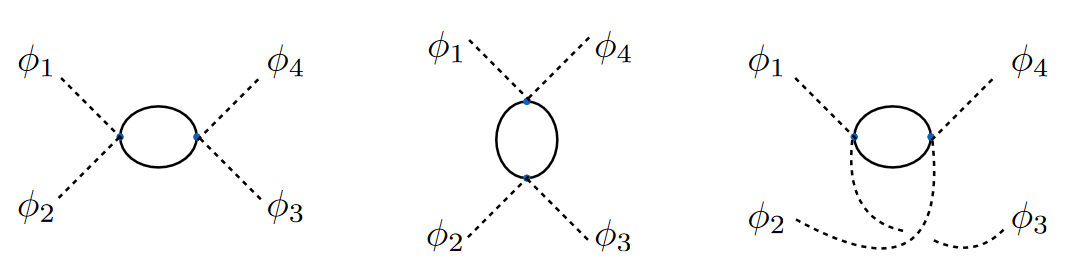
\includegraphics{2019/02/20190212_skinnerquartic.png}
\end{center}
which correspond to an amplitude
\begin{equation}
    \frac{\lambda^2}{2} \int^\Lambda \frac{d^4k}{(2\pi)^4}\frac{1}{k^2+m^2} \bkt{
        \frac{1}{(p_1+p_2+k)^2 +m^2}
        +\frac{1}{(p_1+p_4+k)^2+m^2}
        +\frac{1}{(p_1+p_3+k)^2+m^2}
    }.
\end{equation}
The overall factor of $1/2$ is a symmetry factor since the two internal lines are identical and can be exchanged, and the propagators can be read off by conservation of momentum at each vertex (taking all external momenta to be flowing in). We see that this integral goes as $d^4k/k^4$, so we expect a $\log\Lambda$ divergence. More precisely, the large $k$ behavior (where we care about this divergence) will look like%
    \footnote{This integral isn't totally immediate. To evaluate this, rewrite $k^3 dk= \frac{1}{2}k^2 d(k^2)$. Next, divide through in the numerator and denominator by $m^4$ to get
    \begin{equation*}
        \frac{1}{2}\int_0^\Lambda \frac{(k^2/m^2) d(k^2/m^2)}{(k^2/m^2) +1)^2}=\frac{1}{2}\int_0^{\Lambda^2/m^2} \frac{u\,du}{(u+1)^2}.
    \end{equation*}
    Finally, to evaluate the $u$ integral, just integrate by parts. Some similar integrals like $\int \frac{u\, du}{1+u}$ are amenable to a simple rewriting as $\frac{u}{1+u}=1-\frac{1}{1+u}$, but in general you'll want to integrate by parts:
    \begin{equation*}
        \int_0^{\Lambda^2/m^2} u\frac{du}{(1+u)^2}= -\left.\frac{u}{1+u}\right\rvert_0^{\Lambda^2/m^2} -\int \paren{-\frac{1}{1+u}}du=-\left.\frac{u}{1+u}\right\rvert_0^{\Lambda^2/m^2} +\left.\log(1+u)\right\rvert_0^{\Lambda^2/m^2}=\log\paren{1+\frac{\Lambda^2}{m^2}}-\frac{\Lambda^2}{\Lambda^2+m^2}.
    \end{equation*}
    
    }
\begin{align}
    \frac{3\lambda^2}{2} \int^\Lambda \frac{d^4k}{(2\pi)^4}\frac{1}{(k^2+m^2)^2} &= \frac{3\lambda^2}{16\pi^3} \int_0^\Lambda \frac{k^3 dk}{(k^2+m^2)^2}\\
    &= \frac{3\lambda^2}{32\pi^2} \int_0^{\Lambda^2/m^2} \frac{u\,du}{(1+u)^2}\\
    &= \frac{3\lambda^2}{32\pi^2} \bkt{
        \log\paren{1+\frac{\Lambda^2}{m^2}}-\frac{\Lambda^2}{\Lambda^2+m^2}\label{quarticdivergence}
    }.
\end{align}
This value is the shift in the $\lambda$ coupling before we introduce the $\delta \lambda$ counterterm.
If we then choose
\begin{equation}
    \delta \lambda =\frac{3\lambda^2}{32\pi^2} \bkt{\log \frac{\Lambda^2}{m^2}-1},
\end{equation}
we can then produce an effective coupling of 
\begin{equation}
    \lambda_{\text{eff}}=\lambda -\frac{3\lambda^2}{32\pi^2} \bkt{\log \paren{1+\frac{m^2}{\Lambda^2}}+\frac{m^2}{m^2+\Lambda^2}},
\end{equation}
which is finite as $\Lambda\to\infty$.%
    \footnote{
        This is just $\lambda$ plus the one-loop correction we computed to be \ref{quarticdivergence} plus our choice of $\delta \lambda$ (which is itself treated as a one-loop correction). In fact, we've neglected an overall minus sign in computing the one-loop correction. We should add a factor of $-i$ for the loop, and get rid of the $i$ as part of the overall momentum-conserving delta function which we've already dropped. Thus
        \begin{align*}
            \lambda_\text{eff}&=\lambda -\frac{3\lambda^2}{32\pi^2} \bkt{
                \log\paren{1+\frac{\Lambda^2}{m^2}}-\frac{\Lambda^2}{\Lambda^2+m^2}
            }
            +\frac{3\lambda^2}{32\pi^2} \bkt{\log \frac{\Lambda^2}{m^2}-1}\\
            &= \lambda -\frac{3\lambda^2}{32\pi^2} \bkt{\log \paren{1+\frac{m^2}{\Lambda^2}}+\frac{m^2}{m^2+\Lambda^2}}.
        \end{align*}
    }

For this next discussion, we'll need a trick due to Feynman:
\begin{equation}
    \int_0^1 \frac{dx}{\bkt{xA+(1-x)B}^2} =\frac{1}{B-1} \bkt{\frac{1}{xA+(1-x)B}}_0^1 = \frac{1}{AB}.
\end{equation}
We'll use this to rewrite products of denominators as these sorts of integrals, i.e. from right to left. Note that the integral can be put in a more manifestly symmetric form as
\begin{equation*}
    \int_0^1 dx \int_0^1 dy \frac{\delta(x+y-1)}{(xA+yB)^2}.
\end{equation*}

For our first diagram, let $p_{12}\equiv p_1 +p_2$. Then the propagators take the form
\begin{align*}
    \frac{1}{(p_{12}+k)^2+m^2}\frac{1}{k^2+m^2}&=\int_0^1 \frac{dx}{\bkt{x((p_{12}+k)^2+m^2)+(1-x)(k^2+m^2)}^2
    }\\
        &= \int_0^1 \frac{dx}{\bkt{(k+xp_{12})^2 +m^2 +x(1-x)p_{12}^2}^2}\\
        &= \int_0^1 \frac{dx}{\bkt{l^2+m^2+x(1-x)p_{12}^2}^2}
\end{align*}
where we have defined $l=k+x p_{12}.$
In the $\Lambda \to \infty$ limit, the shifted integration range $|k|\leq \Lambda \to |l|\leq \Lambda$ vanishes, so we can turn our $d^4k$ integral into a $d^4 l$ and write
\begin{align*}
    \int \frac{d^4ldx}
    {\bkt{l^2+m^2+x(1-x)p_{12}^2}^2}
    &= S_4 \int_0^1 dx \int_0^\Lambda \frac{l^3 dl}
    {\bkt{l^2+m^2+x(1-x)p_{12}^2}^2}\\
    &= \pi \int_0^1 dx \set*{ \log \bkt{
        \frac{\Lambda^2 +m^2+x(1-x)p_{12}^2}{m^2+m^2+x(1-x)p_{12}^2}
    }
    +\frac{m^2+x(1-x)p_{12}^2}{\Lambda^2+m^2+x(1-x)p_{12}^2}
    -1
    }
\end{align*}
after a change of variables and an integration by parts. Note that this term with the $1/\Lambda^2$ goes to zero as $\Lambda\to\infty$. Let's notice that all three diagrams are related by the Mandelstam variables 
\begin{equation}
    s=-(p_1+p_2)^2,t=-(p_1+p_4)^2,u=-(p_1+p_3)^2,
\end{equation}
so that the sum of our three diagrams is then
\begin{equation}
    \frac{\lambda^2}{32\pi^2}\int_0^1 dx \set*{ \log \paren{\frac{\Lambda^2}{m^2-x(1-x)s}} 
    + \log \paren{\frac{\Lambda^2} {m^2-x(1-x)t}}
    + \log \paren{\frac{\Lambda^2} {m^2-x(1-x)u}}
    -3
    }.
\end{equation}
The coefficient of $\tilde \phi^4$ in the effective action $\Gamma(\tilde \phi)$ (i.e. $\tilde \phi$ in momentum space) is
\begin{equation}
    \lambda+\delta \lambda -\frac{\lambda^2}{32\pi^2} \int d \set{\ldots}
\end{equation}
with $\delta \lambda$ from above, and replacing $(m^2,\lambda)\mapsto (m_{\text{phys}}^2,\lambda_{\text{eff}})$.
We find that 
\begin{equation}
    \lambda_{\text{eff}}+\frac{\lambda_{\text{eff}}^2}{32\pi^2} \int_0^1 dx \set*{ \log \bkt{1-\frac{x(1-x)s}{m_{\text{phys}}^2}}
    +\log \bkt{1-\frac{x(1-x)t}{m_{\text{phys}}^2}}
    +\log \bkt{1-\frac{x(1-x)u}{m_{\text{phys}}^2}}
    }
\end{equation}
is finite-- no more counterterms are necessary after $\delta m^2$ and $\delta \lambda$. Our capacity to regulate these terms depends on the idea of operators being relevant, irrelevant, or marginal (depending on their mass dimension as compared to the dimension of spacetime).

\section{Thursday, February 14, 2019}
    We've been looking at supersymmetric nonlinear sigma models. Previously, our fields were maps from $x:M\to N$ where $M$ was a worldline and $N$ was some target space, a Riemannian manifold with a metric $g$. But it's clear that $M$ could be some bigger manifold, in general ``our universe.''

We said the Hilbert space for our theory was
\begin{equation}
    \cH = \cH_x \otimes \cH_\psi = \Omega^\cdot (N,\CC),
\end{equation}
the space of differential forms up to $p$-forms on $N$ equipped with inner product
\begin{equation}
    \braket{\alpha}{\beta} = \int_N \bar \alpha \wedge * \beta,
\end{equation}
where $*$ is the Hodge star operator taking $\Omega^p(N)\to \Omega^{n-p}(N)$. Explicitly, if 
\begin{equation*}
    \omega=\omega_{a_1a_2\ldots a_p}dx^{a_1}\wedge dx^{a_2}\wedge \ldots \wedge dx^{a_p},
\end{equation*} then $*\omega$ is given by
\begin{equation*}
    *\omega =\frac{\sqrt{g}}{(n-p)!} \epsilon^{a_1\ldots a_p}{}_{b_{p+1} \ldots b_n} \omega_{a_1\ldots a_p} dx^{b_{p+1}}\wedge \ldots \wedge dx^{b_n},
\end{equation*}
with indices raised by the inverse metric. We saw that our SUSY operator $Q$ then has the geometric interpretation of an exterior derivative,
\begin{equation}
    \hat Q = i\hat{\bar \psi}^a \hat p_a \leftrightarrow d,
\end{equation}
and similarly $\hat{\bar Q}$ has the interpretation of the adjoint of the exterior derivative,
\begin{equation}
    \hat {\bar Q} = -i\hat{ \psi}^a \hat p_a \leftrightarrow d^\dagger,
\end{equation}
where $\avg{\alpha,d^\dagger \beta}=\avg{d\alpha,\beta}$.

We can now fix the ordering ambiguity in $|hat H$ by demanding the SUSY algebra
\begin{equation}
2\hat H=\set{\hat Q,\hat{\bar Q}}
\end{equation}
still holds in the quantum theory. This fixes
\begin{equation}
    H=\frac{1}{2} (d^\dagger d+ dd^\dagger)=-\frac{1}{2} \Delta,
\end{equation}
where $\Delta$ is the Laplacian acting on forms. Since $d:\Omega^p \to \Omega^{p+1}, d^\dagger: \Omega^p \to \Omega^{p-1},$ it follows that $-\Delta=d^\dagger d+dd^\dagger: \Omega^p \to \Omega^p$.

To see this concretely, when acting on a function $f\in \Omega^0(N)$ (i.e. a zero-form), $d^\dagger$ simply annihilates the function (since there are no $-1$-forms) so we get
\begin{align*}
    -\Delta f &= d^\dagger d f\\
        &= d^\dagger(\p_a f dx^a)\\
        &= *d(*df)\\
        &=*d \paren{
            \frac{\sqrt{g}}{(n-1)!} g^{ab} \p_a f \epsilon_{bc\ldots d} \underbrace{dx^c \wedge \ldots \wedge dx^d}_{n-1}
        }\\
        &=\frac{*}{(n-1)!} \p_m (\sqrt{g}g^{ab} \p_a f) \epsilon_{bc\ldots d} \underbrace{dx^m \wedge dx^c \wedge \ldots \wedge dx^d}_n.
\end{align*}
But we see that there are now $n$ one-forms being wedged together, which means we must have all the $dx^1$ through $dx^n$ in some order. We can rewrite this as a totally antisymmetric tensor, with a factor of $1/g$ the determinant of the metric. Using this fact, our expression becomes
\begin{align*}
    -\Delta f&=\frac{1}{g} \p_b(g^{ab}\sqrt{g} \p_a f)*(dx^1 \wedge \ldots \wedge dx^n)\\
    &= -\frac{1}{\sqrt{g}} \p_a(\sqrt{g} g^{ab} \p_b f).
\end{align*}
What we learn is that the generalized Laplacian acting on forms reduces to the ordinary Laplacian with respect to the metric when acting on functions.

However, we now observe that acting on any form $\omega$, 
\begin{align*}
    2\bra{\omega} \hat H \ket{\omega} &= \braket{\omega}{dd^\dagger \omega} + \braket{\omega}{d^\dagger d\omega}\\
        &= ||d^\dagger \omega||^2 + ||d\omega||^2 \geq 0.
\end{align*}
A form which has equality here, $\Delta \omega = 0$, is said to be \term{harmonic}. Therefore supersymmetric ground states are in $1:1$ correspondence with $\text{Harm}^\cdot (N) = \oplus_{p=0}^n \text{Harm}^p(N)$, the space of harmonic $0$- through $p$-forms on $N$. Notice that any form $\omega \in \text{Harm}^p$ must be closed ($d\omega=0$) and co-closed ($d^\dagger \omega=0$).

\begin{thm}[Hodge's theorem] The space of harmonic $p$-forms on $N$ is in correspondence with the de Rham $p$-cohomology group,
\begin{equation}
    \text{\emph{Harm}}^p(N) \cong H^p_{dR}(N)
\end{equation}
where
\begin{equation}
    H^p_{dR}(N)=\set{\omega \in \Omega^p(N)\text{ s.t. }d\omega=0}/\set{\omega=d\alpha} = \text{\emph{ker}}(d:\Omega^p\to \Omega^{p+1})/\text{\emph{im}}(d:\Omega^{p-1}\to \Omega^p).
\end{equation}
\end{thm}
In de Rham cohomology, $\omega$ is specified up to $\omega \sim \omega +d\alpha$ (i.e. we only care about $\omega$ up to the addition of some exact $d\alpha$). The role of the co-closure condition, $d^\dagger \omega=0$, is to select a unique representative. If $d\omega = d^\dagger \omega=0$, then we our freedom becomes $\omega \sim \omega +d\alpha$ where $d^\dagger d\alpha =0$, and the only solutions are $\alpha=0$.%
    \footnote{This is equivalent to the procedure in electromagnetism where we have a potential with a gauge symmetry $A\sim A+d\lambda$, and we fix the gauge by requiring that $d^\dagger A = \p^\mu A_\mu =0$.}
Thus the space of SUSY ground states is $\cong H^\cdot_{dR}(N)$.

Thinking back to our discussion of the Witten index, we see that
\begin{equation}
    I_W = \Tr((-1)^F e^{-\beta H}) = n_B -n_F =\sum_{p=0}^n (-1)^p \dim(H^p_{dR}(N)).
\end{equation}
But this is very interesting because this final expression is precisely $\chi(N)$, the \term{Euler character} of $N$. Thus the space of SUSY ground states has a close relation to some topological information about the space our states live in.

To motivate de Rham cohomology a bit more, suppose $C_p$ is a $p$-cycle in $N$ without boundary. Stokes's Theorem in the vector calculus language says that 
\begin{equation*}
    \int_S(\curl \vec A) \cdot d\vec S=\oint_C \vec A \cdot d\vec l.
\end{equation*}
But we can generalize this to $p$-forms:
\begin{equation}
    \int_{D_{p+1}} d\omega = \int_{C_p} \omega
\end{equation}
if $\p D_{p+1}=C_p$. That is, we can relate the integral in some region $D_{p+1}$ to the value of the form integrated over the boundary $C_p$. However, if $\omega\in H^p_{dR},$ then $d\omega=0 \implies \int \omega=0$ if $C_p$ is the boundary of some $D_{p+1}$.

Furthermore,
\begin{equation}
    \int_{C_p} \omega +d\alpha =\int_{D_{p+1}} d\omega + \int_{D_{p+1}} d^2 \alpha,
\end{equation}
where this second term vanishes since $d$ is nilpotent. Thus we arrive at de Rham's theorem:
\begin{thm}[de Rham]
    \begin{equation}
        H_{dR}^p(N) \cong H_p(N),
    \end{equation}
    where $H_p(N)$ denotes the $p$th homology group, the set \{$p$-cycles in $N$ with no boundary$\}/\{p$-cycles that are the boundary of some $(p+1)$-cycle\}.
\end{thm}

For instance, if $N=S^n$, then $\dim(H_{dR}^0(S^n))=1$. We can also find that  $\dim(H^p_{dR}(S^n))=0$ for $p\neq 0,n$ since we can contract any loop (e.g. an $S^1$) to a point on $S^n$. And then we have $\dim(H^n_{dR}(S^n))=1$, i.e. there is one non-trivial  ``wrapping'' of $S^n$ by an $S^n$.

For $n=\Sigma_g$ a handlebody with genus $n$ (i.e. $n$ donuts glued together) we have instead $H^0(\Sigma_g)=\CC$, $H^1(\Sigma_g)=\CC^{2g}$ and $H^2(\Sigma_g)=\CC$ (dimensions $1,2g,$ and $1$).

The Euler character for the $n$-sphere is
\begin{equation}
    \chi(S^n)=\begin{cases}
        2 & \text{if $n$ even}\\
        0 & \text{if $n$ odd},
    \end{cases}
\end{equation}
and for $\Sigma_g$ it is $\chi(\Sigma_g)=2-2g$.

For the path integral, $\chi(N)=\int e^{-S[x,\psi}\cD x \cD \psi \cD \bar \psi$, where all fields are periodic with period $\beta$. Now if we take the whole action, we see that our whole action is supersymmetrically trivial:
\begin{align}
    S &= \int \frac{1}{2} g_{ab} \dot x^a \dot x^b+\frac{1}{2} g_{ab} \bar \psi^a \nabla_t \psi^b + \frac{1}{4} R_{abcd} \bar \psi^a \psi^b \bar \psi^c \psi^d dt\\
    &= \bar Q \bkt{ \oint \frac{g_{ab} \bar \psi^a}{2}(i\dot x^b +\Gamma^b_{cd} \bar \psi^c \psi^d) dt.}
\end{align}
We therefore learn that the path integral is independent of $\beta$.

\section{Saturday, February 16, 2019}
    Last time, we computed an effective coupling $g_{\text{eff}}$ to be
\begin{equation*}
    g_{\text{eff}}(\mu)=g(\mu)-\frac{3g^2(\mu)}{32\pi^2} \log \frac{\mu^2}{m^2}+\ldots,
\end{equation*}
and in particular since $g_{\text{eff}}$ is the coefficient of $\frac{1}{4!}\phi^4$ in the quantum effective action $\Gamma[\phi]$, it should be independent of $\mu$. Thus
\begin{align}
    0&=\frac{dg_{\text{eff}}}{d\log \mu}\\
        &= \mu\frac{dg_{\text{eff}}}{d\mu}\\
        &=\mu \frac{d}{d\mu} \bkt{g(\mu)-\frac{3g^2(\mu)}{32\pi^2} \log \frac{\mu^2}{m^2}
        }.
\end{align}
This tells us the ``running'' of the renormalized coupling $g(\mu)$, which we refer to as the \term{beta function},%
    \footnote{
        It takes a little algebra to get here. Explicitly, we have
        \begin{align*}
            \beta(g) \equiv \mu \frac{dg}{d\mu}&= \mu \frac{d}{d\mu}\bkt{ \frac{3g^2(\mu)}{32\pi^2} \log \frac{\mu^2}{m^2}
            }\\
            &=\mu \bkt{\frac{3(2g'(\mu) g(\mu))}{32\pi^2} \log \frac{\mu^2}{m^2}
            +\frac{3g^2}{32\pi^2} \paren{\frac{2}{\mu}}
            }\\
            &= \frac{3g}{16\pi^2}\log \frac{\mu^2}{m^2} \paren{\mu \frac{dg}{d\mu}}-\frac{3g^2}{16\pi^2},
        \end{align*}
        so rearranging we find that
        \begin{equation*}
            \mu \frac{dg}{d\mu}=\frac{3g^2}{16\pi^2} \paren{1-\frac{3g}{16\pi^2}\log \frac{\mu^2}{m^2}}= \frac{3\hbar g^2}{16\pi^2}+O(\hbar^2),
        \end{equation*}
        restoring $\hbar$.
    }
\begin{equation}\label{phi4betafunction}
    \beta(g)\equiv \mu\frac{dg}{d\mu}=\frac{3\hbar g^2}{16\pi^2} + O(\hbar^2),
\end{equation}
restoring $\hbar$ which counts the loop order of the corrections. Note that $\beta(g)>0$ for this coupling in this theory.

Integrating the ODE \ref{phi4betafunction} for $\frac{dg}{d\mu}$ between $\mu,\mu'$, we find that
\begin{align}
    \frac{1}{g(\mu')}={}&\frac{1}{g(\mu)}+\frac{3\hbar}{16\pi^2} \log\frac{\mu}{\mu'}\\
    &\implies g(\mu')=\frac{g(\mu)}{1+\frac{3\hbar g(\mu)}{16 \pi^2} \log \frac{\mu}{\mu'}} = g(\mu)-\frac{3\hbar g^2(\mu)}{16\pi^2} \log\frac{\mu}{\mu'}+O(\hbar^2).
\end{align}
For $\mu'>\mu,$ we see that $g(\mu')>g(\mu)$. Note that there is a special scheme-dependent mass scale $\Lambda_{\phi^4}$ such that when $\mu'\to \Lambda_{\phi^4}, g(\mu')\to \infty$. For our scheme, this happens when
\begin{equation}
    \frac{3\hbar g(\mu)}{16\pi^2} \log \frac{\mu}{\Lambda_{\phi^4}} = -1
\end{equation}
at one loop. Thus, knowing this scale allows us to write our coupling as
\begin{equation}
    g(\mu)=\frac{16\pi^2}{3\hbar} \frac{1}{\log(\Lambda_{\phi^4}/\mu)}.
\end{equation}
Exchanging our dimensionless coupling for a dimensionful scale ($\Lambda_{\phi^4}$) is called \term{dimensionful transmutation.} All we're saying is that $\Lambda_{\phi^4}$ is the scale at which perturbation theory breaks down-- perturbation theory works for $\mu \ll \Lambda_{\phi^4}.$

\subsection*{Quantum electrodynamics}
We'll begin our discussion of QED and the photon in the path integral formalism (cf. Skinner Ch. 5, Peskin \& Schroeder). In Euclidean space, we have the classical action
\begin{equation}
     S[\psi,\bar \psi,A]=\int d^4x \bkt{\frac{1}{4} F_{\mu\nu}F^{\mu\nu} + i\bar \psi(\slashed{D}+m)\psi}
\end{equation}
where $\slashed{D}=\gamma^\mu(\p_\mu - ieA_\mu)$ is a covariant derivative and $\psi,\bar \psi$ are four-spin-component Grassmann fields. $F_{\mu\nu}=\p_\mu A_\nu - \p_\nu A_\mu$ is just the electromagnetic field strength tensor.

The partition function for our theory is
\begin{equation}
    Z=\int \cD \psi \cD \bar \psi \cD A \, e^{-S[\psi,\bar \psi,A]}.
\end{equation}
Let us consider the first novel feature of our theory, the electromagnetic field. We write the Fourier transform
\begin{equation}
    A_\mu(x)=\int \frac{d^4k}{(2\pi)^4} e^{ik\cdot x}\tilde A_\mu(k).
\end{equation}
A few steps of algebra%
    \footnote{}
reveals that
\begin{equation}
    \frac{1}{4}\int d^4x F_{\mu\nu}F^{\mu\nu} = \frac{1}{2}\int\frac{d^4k}{(2\pi)^4} \tilde A_\mu(-k)(k^2\delta^{\mu\nu}-k^\mu k^\nu)\tilde A_\nu(k),
\end{equation}
where derivatives have brought down $k$s and the integral over $d^4x$ has related the momenta in $\tilde A_\mu,\tilde A_\nu$.

Note that for a field $\tilde A_\mu(k)=k_\mu \tilde \alpha(k)$ with $\tilde \alpha$ a scalar function, this integral vanishes. This is bad-- since $\int d^4x F_{\mu\nu} F^{\mu\nu}$ is in the action $S$, any path integral configuration of this form will pick up a weight of $1$ from $e^{-S[\psi,\bar\psi,A]}=e^0=1$, and there are infinitely many such configurations to integrate over in $\cD A$, so $Z$ diverges. In position space, this choice of $\tilde A_\mu$ corresponds to $A_\mu(x)=\p_\mu\alpha(x)$.
Recall that under gauge transformations,
\begin{equation}
    A_\mu(x)\mapsto A_\mu(x) +\frac{1}{e} \p_\mu \alpha(x).
\end{equation}
Therefore these troublesome modes are all gauge-equivalent to $A_\mu(x)=0$, and so the solution will come from a gauge fixing procedure.

\subsection*{Faddeev-Popov method for gauge-fixing} Before we do the whole procedure, let's take a simple example. Consider a function $f:\RR^2\to \RR$ that is rotationally invariant,
\begin{equation}
    f(r;\rho)\text{ with }r^2=x^2+y^2,\rho\text{ another parameter}.
\end{equation}
Consider the integral
\begin{align*}
    Z(\rho)&=\int d^2x\, f(r;\rho)\\
        &= \int_0^{2\pi} d\phi \int rdr f(r;\rho) =2\pi \int dr\, r f(r;\rho),
\end{align*}
where we used a change of coordinates to do the integral. Easy enough to compute. We separated and integrated out a trivial part of the integral, the $d\phi$ part, leaving only the interesting $r$ dependence.

But there's another way to think about this integration.%
    \footnote{Following Skinner's conventions (Ch. 8 of his notes), I've significantly rewritten this section from how it was presented in class in anticipation of later gauge fixing content.}
Consider an integration path given by the constraint $g(\vec x)=0$ for some function of our choosing $g(\vec x)$. We may (following Skinner) call this path a \term{gauge slice} and the function a \term{gauge-fixing function}. In particular, let's say we want to integrate only along the $x$-axis, i.e. $g(\vec x)=y=0$. Consider then the related integral
\begin{equation}
    \int d^2x \, \delta(g(\vec x)) f(r;\rho).
\end{equation}
With the delta function, this integral does what we wanted-- it restricts the integration path precisely to $g(\vec x)=0$. However, its value clearly depends on our choice of path, since rescaling $g\to cg$ for some constant $c$ will rescale the entire integral by a factor $1/|c|$. This is because the $\delta$ function changes with our gauge fixing function $g$. However, we can account for this as follows. We introduce the factor
\begin{equation}
    \Delta_g (\vec x)=\left.\P{}{\theta}g(R_\theta \vec x)\right|_{\theta=0}
\end{equation}
where $R_\theta$ indicates that we rotate our coordinates by an angle $\theta$ before evaluating our gauge fixing function $g(\vec x)$. This factor precisely captures how the delta function changes as we change $g$ by an infinitesimal rotation, so that the integral
\begin{equation}
    \int d^2x \abs{\Delta_g(\vec x)} \delta(g(\vec x)) f(r;\rho)
\end{equation}
is now independent of both reparametrization of $g$ and rotations by $\theta$. In fact, notice that so long as our gauge slice only hits each gauge orbit once, the integral is completely independent of the gauge slice. For our example, it is straightforward to compute $\Delta_g(\vec x)$:
\begin{equation}
    \Delta_g(\vec x) = \P{}{\theta}(y\cos\theta - x\sin\theta)|_{\theta=0}= -y\sin\theta -x\cos\theta|_{\theta=0}=-x.
\end{equation}

To see how this factor emerges, consider again our delta function $\delta(g(\vec x))=\delta(y)$. Under a rotation by $\theta$, $y\mapsto y_\theta = y\cos\theta -x\sin\theta$, so
\begin{equation}
    \delta(y) \mapsto \delta(y_\theta) = \delta(y\cos\theta-x\sin\theta).
\end{equation}
Let us now write this delta function in terms of $\theta$ using the composition rule of the $\delta$ function: for a function $f$ with a single zero $f(x_0)=0$, $\delta(f(x))=\frac{\delta(x-x_0)}{|f'(x_0)|}$. Thus
\begin{equation}
    \delta(y_\theta)=\frac{\delta(\theta-\tan^{-1}\frac{y}{x})}{\abs{y\sin\theta +x\cos\theta}_{\theta=0}}=\frac{\delta(\theta-\tan^{-1}\frac{y}{x})}{|x|}.
\end{equation}
By definition, when $\tan^{-1} y/x \in (0,\pi),$ the delta function satisfies
\begin{align*}
    1 &= \int_0^\pi d\theta\, \delta(\theta-\tan^{-1}\frac{y}{x})\\
        &= \int_0^\pi d\theta \, \delta(y\cos\theta-x\sin\theta)\abs{x}\\
        &= \int_0^\pi d\theta\, \delta(y_\theta) \abs*{\P{y_\theta}{\theta}}.
\end{align*}
We recognize $\abs*{\P{y_\theta}{\theta}}=\Delta_g(\vec x)$. Then
\begin{equation}
    Z(\rho)=\int d^2x \int_0^\pi d\theta\, \delta(y_\theta) \abs*{\P{y_\theta}{\theta}} f(r;\rho).
\end{equation}
The factor of $\abs*{\P{y_\theta}{\theta}}$ is a simple example of a \term{Faddeev-Popov determinant}, which we have already met in \emph{String Theory}.

We are now free to change integration variables $y\to y_\theta$ and relabel to $y$ so that our integral becomes
\begin{equation}
    Z(\rho) = \int d^2x\int_0^\pi d\theta\, \delta(y)\abs*{\P{y}{\theta}}_{\theta=0} f(r;\rho),
\end{equation}
where the integral is now $\theta$-independent.
In particular, notice that
\begin{align*}
    \abs*{\P{y}{\theta}}_{\theta=0} =|x| \implies Z(\rho) &= \pi \int_{\RR^2} d^2x \,\delta(y) |x| f(r;\rho)\\
    &= 2\pi \int_0^\infty dx\, x f(x;\rho)
\end{align*}
as before.
If we had $N$ variables and $N-1$ rotations with angles $\theta_{1i},i=2,\ldots, N$, then we would have instead the determinant
\begin{equation}
    1=\int d\theta_{1i} \delta(x_{\theta i}^i) \abs*{\frac{dx_{\theta_{1i}}^i}{d\theta_{1i}}}.
\end{equation}

This approach generalizes-- in our gauge theory, we fix the gauge with some functional of $A_\mu(x)$, i.e. $G[A]=0$. For example, $G[A]=\p_\mu A^\mu$ in Lorenz [sic] gauge. Consider now gauge transformations
\begin{equation}
    A_\mu^\alpha(x)=A_\mu (x) +\frac{1}{e} \p_\mu \alpha(x).
\end{equation}
We now use the identity
\begin{equation}
    1= \int \cD \alpha(x) \delta (G[A]) \det \paren{\frac{\delta G[A]}{\delta \alpha}},
\end{equation}
where this last factor is a functional determinant. We'll see how the gauge-fixing procedure modifies the photon propagator next time.

\subsection*{Non-lectured aside: on Fadeev-Popov determinants}

Let us briefly remark on what we've done. We had a theory over some potentially complicated space, but we recognized that there was a redundancy in our description. In the case of our rotationally invariant integral, we saw that on $r={}$constant orbits, the integrand was also constant. This led us to take a gauge slice, i.e. to fix a path through the space which only intersects each gauge orbit once, and then multiply by the ``size'' of a gauge orbit. More generally, the ``size'' of a gauge orbit will be infinite, but we can still use this method to choose a gauge slice in our configuration space, and we include the Faddeev-Popov determinant to ensure that the integral is independent of our choice of path.

The way it was presented in lecture is a bit backwards from how we use this method. Here is a quick recap of how we will use this.
\begin{enumerate}
    \item Identify a gauge symmetry of the theory.
    \item Identify the gauge orbits.
    \item Choose a gauge-fixing function such that $g=0$ along the gauge slice (integration path).
    \item Calculate the Faddeev-Popov determinant, i.e. compute the variation of $g$ as we go around a gauge orbit, evaluated at our gauge slice.
    \item Insert the delta function and the Faddeev-Popov determinant into the integral.
    \item Perform the integral using the delta function.
\end{enumerate}
How does this connect to our example?
\begin{enumerate}
    \item We identified an $SO(2)$ gauge symmetry.
    \item We identified the gauge orbits as sets of constant $r$, and within each orbit there was a gauge freedom described by $\theta$.
    \item We chose as our gauge-fixing function $g=y$.
    \item We calculated the Faddeev-Popov determinant by varying with respect to the parameter $\theta$ describing the gauge freedom: $\Delta_g (\vec x)=\left.\P{}{\theta}g(R_\theta \vec x)\right|_{\theta=0}=-x$.
    \item We insert the delta function $\delta(y)$ and the Faddeev-Popov determinant into our integral to get $\int d^2x \,\delta(y)|x| f(r;\rho)= \int_{-\infty}^\infty dx \, |x| f(x;\rho)$.
\end{enumerate}

\section{Tuesday, February 19, 2019}
    Last time, we wrote down an action for the electromagnetic field,
\begin{equation*}
    S_g[A]=\frac{1}{4}\int d^4x F_{\mu\nu}F^{\mu\nu} = \frac{1}{2}\int\frac{d^4k}{(2\pi)^4} \tilde A_\mu(-k)(k^2\delta^{\mu\nu}-k^\mu k^\nu)\tilde A_\nu(k),
\end{equation*}
We introduced the Faddeev-Popov method for fixing the gauge. We write the identity in terms of a delta function and an (as yet unspecified) functional $G[A]$,
\begin{equation*}
    1= \int \cD \alpha(x) \delta (G[A]) \det \paren{\frac{\delta G[A]}{\delta \alpha}}.
\end{equation*}

For the $G[A]$ we will use, the determinant (Jacobian factor) will be independent of $A$, though this will not be true more generally in non-Abelian gauge theories. We can denote the gauge-transformed $A$ as
\begin{equation}
    A_\mu^\alpha(x)=A_\mu (x) +\frac{1}{e} \p_\mu \alpha(x).
\end{equation}
If we choose to work in Lorenz gauge, for example, then
\begin{equation}
    G[A]=\p_\mu A^\mu \implies G[A^\alpha]=\p_\mu A^\mu +\frac{1}{e} \p^2 \alpha,
\end{equation}
so
\begin{equation}
    \det \paren{\frac{\delta G[A]}{\delta \alpha}}=\det \paren{\frac{\p^2}{e}}.
\end{equation}
%what does this mean, notationally?
Thus we rewrite the path integral with our delta function as
\begin{align}
    \int \cD A e^{-S_g[A]} &= \det \paren{\frac{\delta G[A^\alpha]}{\delta \alpha}} \int \cD \alpha \int \cD A e^{-S_g[A]} \delta(G[A])\\
    &=\det \paren{\frac{\delta G[A^\alpha]}{\delta \alpha}} \paren{\int \cD \alpha} \int \cD A e^{-S_g[A]} \delta(G[A]),
\end{align}
where we have changed variables $A\mapsto A^\alpha$, and $S_g$ is invariant since this is a gauge transformation.%
    \footnote{n.b. this path integral over gauge transformations $\int \cD \alpha$ is infinite. It is the same infinity that cropped up when we tried to naively compute the full path integral before gauge fixing, but here we have isolated it with our gauge fixing procedure so it can be readily discarded.}

To fix the gauge, let's choose the functional
\begin{equation}
    G[A]=\p_\mu A^\mu(x) -\omega(x) \implies G[A^\alpha]=\p_\mu A^\mu - \omega +\frac{1}{e} \p^2 \alpha.
\end{equation}
We now integrate over $\omega$ with a Gaussian weight factor of mean $0$ and variance $\xi$. Thus
\begin{equation}
    \int \cD \omega \exp \bkt{-\int d^4x \frac{\omega^2}{2\xi}} \det \paren{\frac{\p^2}{e}} \int \cD \alpha \cD A e^{-S[A]}\delta(\p_\mu A^\mu -\omega),
\end{equation}
which becomes (similar to before)
\begin{equation}
    \det \paren{\frac{\p^2}{e}} \paren{\int \cD \alpha} \int \cD A e^{-S_g[A]}\exp \bigg(-\underbrace{\int d^4x \frac{1}{2\xi}(\p_\mu A^\mu)^2}_{S_{gf}[A]}\bigg),
\end{equation}
where $S_{gf}$ indicates a gauge-fixing action. Thus
\begin{equation}
    S_g[A]+S_{gf}[A]=\frac{1}{2} \int \frac{d^4k}{(2\pi)^k} \tilde A_\mu(-k) \bkt{k^2 \delta^{\mu\nu}-(1-\frac{1}{\xi})k^\mu k^\nu} \tilde A_\nu(k),
\end{equation}
where we've just taken a Fourier transform as usual. The propagator solves
\begin{equation}
    (k^2 \delta^{\mu\nu}-(1-\frac{1}{\xi})k^\mu k^\nu)\tilde D_{\nu\rho}(k)=\delta^\mu{}_\rho,
\end{equation}
so the photon propagator takes the form
\begin{equation}
    \tilde D^{\mu\nu}(k)=\frac{1}{k^2}\paren{ \delta^{\mu\nu}-(1-\xi) \frac{k^\nu k^\nu}{k^2}}.
\end{equation}
Here, $\xi=0$ is known as Lorenz or Landau gauge depending on when the $\xi$ condition is imposed, while $\xi=1$ is known as Feynman gauge.

\subsection*{Free fermions (electrons)}
Let us consider an action in terms of fermions,
\begin{equation}
    S[\psi,\bar \psi]=\int d^4x (-\bar \psi(\slashed{\p}+m)\psi),
\end{equation}
where we work in Euclidean signature, $\slashed{\p}=\gamma_\mu \p^\mu$, and the anticommutation relations hold,
\begin{equation}
    \set{\gamma_\mu,\gamma_\nu}=2\delta_{\mu\nu}.
\end{equation}
Our gamma matrices are hermitian, $\gamma_\mu^\dagger =\gamma_\mu$, and our $\gamma_5$ is taken to be $\gamma_5=\gamma_1 \gamma_2 \gamma_3 \gamma_4$. For example,
\begin{equation}
    \gamma_j=\begin{pmatrix}
        0& -i\sigma_j\\
        i\sigma_j & 0
    \end{pmatrix},
    \quad
    \gamma_4 = \begin{pmatrix}1 & 0 \\ 0 &-1\end{pmatrix}
    \text{ or } \begin{pmatrix}0 & 1 \\ 1 & 0\end{pmatrix}.
\end{equation}

We take the Fourier transform of our fermionic fields using
\begin{gather}
    \psi(x) =\int_p e^{ip\cdot x} \tilde \psi(p),\\
    \bar \psi(x) = \int_p e^{-ip\cdot x} \tilde{\bar \psi}(p)
\end{gather}
where $\int_p = \int \frac{d^4p}{(2\pi)^4}$. Thus in Fourier space our action takes the form
\begin{equation}
    S[\tilde \psi, \tilde{\bar \psi}]= \int_p \tilde{\bar \psi}(i\slashed{p}+m)\tilde \psi.
\end{equation}
Adding sources $\tilde \eta, \tilde{\bar \eta}$, the generating functional is then
\begin{align}
    Z[\tilde \eta,\tilde{\bar \eta}]&=\int \cD \tilde \psi \cD \tilde{\bar \psi} \exp \paren{-\int_p \bkt{ \tilde{\bar \psi}(i\slashed{p}+m)\tilde \psi - \tilde{\bar \eta} \tilde \psi +\tilde {\bar \psi}\tilde \eta}}\\
    &= Z[0,0] \exp\paren{-\int_p \tilde{\bar \eta}(i\slashed{p}+m)^{-1} \tilde \eta},
\end{align}
where we have completed the square as usual.

\subsection*{Feynman rules} In addition to the propagators and vertices, fermion loops pick up minus signs. For instance, the position space propagator takes the form
\begin{equation}
    S_F^{\alpha\beta}(x-y)=\avg{\psi^\alpha(x) \bar \psi^\beta(y)}=\int_p e^{ip \cdot(x-y)} \paren{\frac{1}{i \slashed{p}+m}}^{\alpha\beta},
\end{equation}
where $\alpha,\beta$ are spin indices $1,\ldots,4$. If we expand the action $e^{-S_{QED}}$ to second order in the electron-photon coupling, we find terms
\begin{align*}
    (-ie)^2 \avg{\paren{\int d^4x \bar \psi \slashed{A} \psi}\paren{\int d^4y \bar \psi \slashed{A} \psi}} &= (-ie)^2 \int d^4x d^4 y \,
    \avg{\slashed{A}^{\alpha\beta}(x) \slashed{A}^{\gamma\delta}(y) \bar \psi^\alpha(x) \psi^\beta(x) \bar \psi^\gamma(y) \psi^\delta(y)}.
\end{align*}
In general, we need to anticommute the $\psi$s and $\bar \psi$s to form propagators. One term is
\begin{equation}
    -(-ie)^2\int d^4x d^4y \,
    \paren{
        \slashed{A}^{\alpha\beta}(x) \slashed{A}^{\gamma\delta}(y) \underbrace{\psi^\beta(x) \bar \psi^\gamma(y)}_{S_F^{\beta\gamma}(x-y)} \underbrace{\psi^\delta(y) \bar \psi^\alpha(x)}_{S_F^{\delta \alpha}(y-x)}
    }
\end{equation}
where the overall minus sign comes from anticommuting and we've recognized the pairs $\psi \bar \psi$ as propagators.

We get some Feynman rules for this theory:
%see diagram
\begin{enumerate}
    \item The fermion propagator is an oriented line, with $\tilde S_F(p)=\frac{1}{i\slashed{p}+m}$
    \item The photon propagator is a squiggly line, $\tilde D^{\mu\nu}(k)=\frac{1}{k^2}(\delta^{\mu\nu}-(1-\xi)\frac{k^\mu k^\nu}{k^2})$
    \item The vertex gets a $-ie\gamma^\mu$.
    \item We pick up an overall factor of $(-1)^{l_F},$ where $l_F$ is the number of fermion loops.
\end{enumerate}

\section{Thursday, February 21, 2019}
    Last time, we considered fields in some spacetime and chose Gaussian normal coordinates in order to write (for variations of the fields $x^a=x^a_0+\delta x^a(\tau), \psi^a=\psi^a_0 +\delta \psi^a(\tau)$,
\begin{equation*}
    g_{ab}(x)=\delta_{ab} -\frac{1}{3} R_{acbd} (x_0) \delta x^c \delta x^d + O(\delta x^3)
\end{equation*}
and a connection
\begin{equation*}
    \Gamma^a_{bc}(x) = \p_d \Gamma^a_{bc}(x_0) \delta x^d = -\frac{1}{3} (R^a{}_{bcd}(x_0) +R^a{}_{cbd}(x_0))\delta x^d + O(\delta x^2).
\end{equation*}

So we have the quadratic action
\begin{equation}
    S^{(2)}[x_0,\psi_0,\delta x, \delta \psi]=\oint \paren{-\frac{1}{2} \delta x^a \delta_{ab} \frac{d^2}{d\tau^2}\delta x^b +\frac{1}{2} \delta \psi^a \delta_{ab} \frac{d}{d\tau} \delta \psi^b -\frac{1}{4} R_{abcd} \psi_0^a \psi_0^b \delta x^c \frac{d\delta x^d}{d\tau}} d\tau.
\end{equation}
For any fixed $(x_0^a,\psi_0^a)$, this is a free action, so the path integral over fluctuations gives
\begin{equation}
    \int e^{-S[x_0,\psi_0,\delta x , \delta \psi]}\cD \delta x \cD \delta \psi = \frac{\sqrt{\det'(\p_\tau \delta^b_a)}}{\sqrt{\det'(-\p^2\tau \delta^a_b - \mathcal{R}^a{}_b (x_0,\psi_0)\p_\tau)}}
\end{equation}
where $\mathcal{R}^a{}_b=R^a{}_{bcd}(x_0) \psi_0^c \psi_0^d$ and $\det'$ means without zero modes, i.e. we haven't yet done the integrals over $(x_0,\psi_0).$

We can split up the denominator by pulling out a $\p_\tau$ to find
\begin{equation}
    \int e^{-S[x_0,\psi_0,\delta x , \delta \psi]}\cD \delta x \cD \delta \psi = \frac{\sqrt{\det'(\p_\tau \delta^b_a)}}{\sqrt{\det'(\delta^a{}_b \p_\tau)}\sqrt{\det'(-\delta^a{}_b \p_\tau - \mathcal{R}_a{}^b)}}
    =\frac{1}{\sqrt{\det'(-\delta^a{}_b \p_\tau - \mathcal{R}^a{}_b)}}.
\end{equation}
Notice that the matrix $\mathcal{R}^a{}_b$ is an antisymmetric $n\times n$ matrix (since we contracted over two indices in the original Riemann tensor, and $R^a{}_{bcd}$ was already antisymmetric in the first two indices) and $n=2m$. We therefore decompose the tangent space $TN|_{x_0}$ into $m$ 2-dimensional subspaces on which $\mathcal{R}^a{}_b|_i$ takes the form
\begin{equation}
    \mathcal{R}^a{}_b|_i =\begin{pmatrix} 0 & \omega_i \\ -\omega_i & 0\end{pmatrix}.
\end{equation}
Let $-D_i$ be the restriction of $-\delta^a{}_b \p_\tau -\mathcal{R}^a{}_b$ to this 2D subspace.

We expand
\begin{equation}
    \delta x^a(\tau)=\sum_{k\neq 0} \delta x_k^a e^{2\pi i k \tau}.
\end{equation}
Then the eigenvalues of $-D_i$ on this subspace are $-2\pi i k \pm \omega_i$ for $k\in \ZZ,k\neq 0$ (where the first term comes from acting on a Fourier mode with $\p_\tau$ and the second comes the eigenvalues of $\mathcal{R}^a{}_b|_i$ being $\pm\omega$). Therefore
\begin{align*}
    \det(-D_i)&=\prod_{k\neq 0} (-2\pi i k+\omega_i)(-2\pi i k -\omega_i)\\
    &= \prod_{k\neq 0}(-(2\pi k)^2-\omega_i^2)\\
    &= \prod_{k=1}^\infty (2\pi k)^4 \prod_{k=1}^\infty \paren{1+\frac{\omega_i^2}{(2\pi k)^2}}^2,
\end{align*}
where the rewriting in the last line has come from changing the $k\neq 0$ product to a product over $k=1\to\infty$. 

This is clearly divergent thanks to the first factor. However, we can regularize this, e.g. using zeta-function regularization. We find that
\begin{equation}
    \prod_{k=1}^\infty (2\pi k)^4 = (4\pi^2)^{2\zeta(0)}e^{-2\zeta'(0)}=1.
\end{equation}
The important factor is then
\begin{equation*}
    \prod_{k=1}^\infty \paren{1+\frac{\omega_i^2}{(2\pi k)^2}}^2,
\end{equation*}
and we recall that 
\begin{equation*}
    \sinh(z)=z\prod_{k=1}^\infty \paren{1+\frac{z^2}{\pi^2 k^2}},
\end{equation*}
so after regularization, we have that $z=\omega_i^2/2$ and (by direct comparison with the expansion of $\sinh(z)$) our determinant term can be written as
\begin{equation}
    \sqrt{\det{}'(-D_i)}=\frac{\sinh(\omega_i/2)}{(\omega_i/2)}.
\end{equation}
We now see that
\begin{align}
    I_W&=\text{index}(\slashed\nabla)=\int \prod_{i=1}^\infty \frac{\omega_i/2}{\sinh(\omega_i/2)} d^n x_0 d^n\psi_0\\
        &= \int \det \paren{\frac{\mathcal{R}^a{}_b(x_0,\psi_0)/2}{\sinh(\mathcal{R}^a{}_b}(x_0,\psi_0)/2)}d^n x_0 d^n \psi_0.
\end{align}
where $\slashed{\nabla}$ denotes the Dirac operator on $N$. But by our regular Grassmann tricks, we must have precisely $n$ factors of $\psi_0$ in order for this integral to be non-vanishing. Thus
\begin{equation}
    I_W = \int_N \det \paren{\frac{\mathscr{R}/2}{\sinh \mathscr{R}/2}}.
\end{equation}
where $\mathscr{R}^a{}_b=R^a{}_{bcd}(x) dx^c \wedge dx^d$ is a curvature two-form. This is the Aatiyah-Singer index theorem.

\subsection*{Supersymmetric QFT}
If we had a $d$-dimensional theory that is Lorentz invariant, we must complete the supersymmetry algebra $\set{Q,Q^\dagger}=2H$. The Hamiltonian now comes with nontrivial kinetic terms and is part of the $d$-momentum multiplet $P_\mu$, so we need further supercharges. If we want to preserve $Q^\dagger =(Q)^\dagger$, then these supercharges must have the same spin, and so must each have spin $1/2$.

Specifically, the SUSY algebra in $d$-dimensions is
\begin{equation}
    \set{Q_\alpha,Q_\beta^\dagger}=2\gamma^\mu_{\alpha\beta} P_\mu,
\end{equation}
where $\alpha,\beta$ are spinor indices and $\gamma^\mu$ is a Dirac $\gamma$ matrix. We'll mostly be concerned with $d=2$, where Dirac spinors have $2^{(d/2)}=2$ complex components. Thus we can write $\psi=\begin{pmatrix}\psi_-\\\psi_+\end{pmatrix}$. With coordinates $(t,s)\in \RR^2$ and Minkowski metric $\eta_{\mu\nu}=\text{diag}(+,-)$, we can represent the Dirac $\gamma$s as
\begin{equation}
    \gamma^t = 
    \begin{pmatrix} 
    0 & 1\\
    1& 0
    \end{pmatrix},
    \quad
    \gamma^s = 
    \begin{pmatrix} 
    0 & -1\\
    1 & 0
    \end{pmatrix}.
\end{equation}
These obey the Clifford algebra $\set{\gamma^\mu, \gamma^\nu}=2\eta^{\mu\nu}$. The action for a free, massless Dirac spinor in $d=2$ is then
\begin{equation}
    S[\psi]=\frac{1}{2\pi}\int_{\RR^2} i\bar \psi \slashed{\p} \psi d^2 x
\end{equation}
where $\slashed{\p}=\gamma^\mu \p_\mu$ and $\bar \psi=\psi^\dagger \gamma^t$. We can of course plug in the explicit form of the spinors and $\gamma$ matrices, and we find that
\begin{equation}
    S[\psi]=\frac{1}{2\pi}\int {\RR^2} i\bar \psi_- (\p_t +\p_s)\psi_- +i\bar \psi_+(\p_t-\p_s)\psi_+ dtds,
\end{equation}
so we see that the spinor components decouple. Classically,
\begin{equation}
    (\p_t + \p_s)\psi_-=0\implies \psi_-(t,s)=f(t-s)
\end{equation}
represents a right-moving mode, while
\begin{equation}
    (\p_t - \p_s)\psi_+=0\implies \psi_+(t,s)=f(t+s)
\end{equation}
is a left-moving mode. Under an $SO(1,1)$ transformation, i.e.
\begin{equation}
    \begin{pmatrix}t\\ s\end{pmatrix} \mapsto
    \begin{pmatrix}
    \cosh\gamma & \sinh\gamma\\
    \sinh\gamma & \cosh\gamma
    \end{pmatrix}
    \begin{pmatrix}t\\ s\end{pmatrix}
\end{equation}
with $\gamma$ the usual (real) rapidity, the spinor components transform as
\begin{equation}
    \psi_\pm \mapsto e^{\pm \gamma/2}\psi,\quad \bar\psi_\pm \mapsto e^{\pm \gamma/2}\bar\psi.
\end{equation}

\section{Saturday, February 23, 2019}
    \subsection*{QED counterterms}
Last time, we calculated the vacuum polarization at one loop. There are other loop diagrams we might be interested in, like the electron self-energy and the one-loop correction to the electron-photon interaction (see diagram).

To renormalize our theory, we will add counterterms of the form
\begin{equation}
    S^{CT}[\psi,\bar \psi,A,\epsilon] = \int d^dx \bkt{\frac{\delta Z_3}{4} F_{\mu\nu}F^{\mu\nu} +\delta Z_2 \bar \psi \slashed{D} \psi + \delta m \bar \psi \psi
    }.
\end{equation}
It's this second (gauge invariant) term we'll need in the following calculation. As $d\to 4$ ($\epsilon\to 0$), we have
\begin{equation}
    \pi_{\text{1-loop}}(q^2)=-\frac{g^2(\mu)}{2\pi^2} \int_0^1 dx\, x(1-x)\paren{\frac{2}{\epsilon}-\gamma +\log \frac{4\pi \mu^2}{\Delta}
    } + O(\epsilon)
\end{equation}
with $\Delta,\mu$ as before and $\gamma$ the Euler-Mascheroni constant. In the $\overline{\text{MS}}$ term,
\begin{equation}
    \delta Z_3 = -\frac{g^2(\mu)}{12\pi^2} \paren{\frac{2}{\epsilon}-\gamma +\log 4\pi
    }.
\end{equation}
After renormalization, the 1-loop self-energy takes the form
\begin{equation}
    \pi_{\text{1-loop}}^{\text{ren}}(q^2)=\frac{g^2(\mu)}{2\pi^2} \int_0^1 dx\, x(1-x) \log \paren{\frac{m^2+x(1-x)q^2}{\mu^2}}.
\end{equation}
Thus we've killed off the $1/\epsilon$ divergence and the constants, and have substituted back in $\Delta = m^2+q^2 x(1-x).$
Note the branch cut in this integral for $m^2+x(1-x)q^2 \leq 0,$ when the argument of the $\log$ becomes negative or zero. In fact, there's a physical interpretation for this. For $x\in [0,1]$ we see that $0\leq x(1-x) \leq 1/4$. In Minkowski signature, $q_0=iE$, the branch cut therefore corresponds to
\begin{equation}
    m^2 \leq x(1-x) (E^2-\vec q^2) \leq \frac{1}{4} (E^2-\vec q^2)
\end{equation}
so the smallest $E$ that satisfies this is simply $E^2=(2m)^2$. This is precisely the minimum energy required to create a real (on-shell) electron-positron pair.

\subsection*{QED $\beta$ function}
%revisit this
The simplest way to obtain the beta function for the QED coupling is to rescale the field
\begin{equation*}
    A_\mu \to \frac{A_\mu}{g}
\end{equation*}
so that the action is
\begin{align}
    \frac{1}{4g_{\text{eff}}^2} \int d^4x F_{\mu\nu} F^{\mu\nu} &=\frac{1-\pi_{\text{1-loop}}^{\text{ren}}(0)}{4g^2(\mu)} \int d^4x\, F_{\mu\nu} F^{\mu\nu}\\
        &=\frac{1}{4} \bkt{\frac{1}{g^2(\mu)}-\frac{\hbar}{12\pi^2} \log\frac{m^2}{\mu^2}+O(\epsilon)
        }\int d^4x \, F_{\mu\nu}F^{\mu\nu}.
\end{align}
Then the beta function is
\begin{equation}
    \beta(g)=\frac{\hbar g^3(\mu)}{12\pi^2}+O(\hbar^2)>0.
\end{equation}
Integrating, we can see how $g$ depends on $\mu$: it is
\begin{equation}
    \frac{1}{g^2(\mu')}=\frac{1}{g^2(\mu)}+\frac{\hbar}{6\pi^2}\log\frac{\mu}{\mu'}+ O(\hbar^2).
\end{equation}
Let $\Lambda_{QED}$ be the scale at which the coupling diverges,
\begin{equation}
    g^2(\mu)=\frac{g\pi^2}{\hbar} \frac{1}{\log \Lambda_{QED}/\mu}.
\end{equation}
Given that $m_e=\SI{0.511}{\mega\eV}$, we have a coupling constant $\alpha=\frac{g^2(m_e)}{4\pi}\approx \frac{1}{137}$ (the fine structure constant), which tells us that $\Lambda_{QED}\sim \SI{e286}{\giga\eV}$. Note that at scales $\mu=\SI{100}{\giga\eV},$ the EM and weak forces merge into the electroweak force.

\subsection*{Renormalization group}
Let's begin our discussion of renormalization by remarking that a QFT is not fully defined by its Lagrangian $\cL$ (or equivalently an action $S$). A full definition requires that we regularize the theory in order to tame its divergences, which introduces an associated (unphysical) mass scale. Thus we impose some renormalization conditions in order to uniquely set the parameters of our theory, which requires empirical input (i.e. experiments to set the effective couplings). Once this is done, we can use a QFT to make predictions.

However, the physical predictions of our theory should be independent of arbitrary choices made in defining the theory. That is, the predictions must be the same at low energies independent of regularization scheme. This leads us to a sense of \term{universality}, just as we saw in \emph{Statistical Field Theory}. That is, no matter what is going on in the UV, our effective theory describes the same IR physics emerging from families of theories with different regularization schemes or scales.

The renormalization group is therefore the natural structure to study how theories with different short-distance (UV) details can give rise to the same long-distance (IR) physics.

To see an example of this, consider a real scalar theory in $d$ dimensions with a momentum cutoff $\Lambda_0$.
\begin{equation}
    S_{\Lambda_0}[\phi]=\int d^dx\bkt{
        \frac{1}{2} \p_\mu \phi \p^\mu \phi +\frac{1}{2} m^2 \phi^2 +\sum_i \frac{1}{\Lambda_0^{d_i-d}} g_{i0} O_i(x)
    }
\end{equation}
where $O_i$ are local operators of mass dimension $d_i >0$ made up of fields and their derivatives. For instance,
\begin{equation}
    O_i=(\p\phi)^{r_i} \phi^{s_i}.
\end{equation}
We can count the total number of fields in $O_i$-- call it $n_i$, where in this example $n_i=r_i+s_i$.

The partition function with a cutoff, denoted $\cZ$, is now
\begin{equation}
    \cZ(g_{i0})=\int^{\Lambda_0} \cD \phi e^{-S_{\Lambda_0}[\phi]}.
\end{equation}
This tells us to integrate over fields with $\abs{p} \leq \Lambda_0$.
\end{document}